%Chapter 2

\renewcommand{\thechapter}{2}

\chapter[Alignment and mapping metods]
{Improving accuracy and speed of mapping and alignment methods}
\label{chapt2}

In this chapter, I explore new ideas for improving the alignment and mapping methods. 
In the first part of the chapter, I address some of the existing obstacles with the 
lightweight  alignment approaches. These methods are employed in the recent non-alignment 
based quantfication tools such as salmon~\citep{Patro2017Salmon}, and 
kallito~\citep{Bray2016Kallisto} to map the RNA-seq reads to the set of known reference 
sequences instead of aligning the reads. We show that the accuracy of the lightweight 
quantification methods decline in the difficult cases which often exist in the real 
samples. We introduce a new algorithm for selectively aligning RNA-seq reads to a 
transcriptome, with the goal of improving transcript-level quantification in adversarial 
scenarios.
\footnote{This is a joint project with Hirak Sarkar and is presented in BCB 2017~\citep{selaln}}

Furthermore, in the second section of this chapter, we build upon the idea of selective 
alignment to introduce Puffaligner~\citep{almodaresi2021puffaligner}, an all purpose 
aligner for short read sequencing reads which can be used in many cases ranging from 
alignment of RNA-seq, DNA-seq and metagenomic samples to known set of references. 
Puffaligner indexes the reference sequences using the Pufferfish index~\citep{pufferfish} 
which efficiently indexes the \cdbg built from the reference sequences.\footnote{This is 
a joint project with Fatemeh Almodaresi and is published in 
Bioinformatics~\citep{almodaresi2021puffaligner}}


\section{Towards Selective Alignment}

While alignment is a staple of many genomic analyses, it sometimes represents more 
information than is actually necessary to address the analysis at hand. For example, 
recent tools like \sailfish~\citep{Patro2014Sailfish}, \rnaskim~\citep{zhang2014rna}, 
\kallisto~\citep{Bray2016Kallisto}, \salmon~\citep{Patro2017Salmon}, and 
\fleximer~\citep{ju2017fleximer}, demonstrate that accurate quantification estimates can 
be obtained without all of the information encoded in traditional alignments. By avoiding 
traditional alignment procedures, these tools are much faster than their alignment-based 
counterparts. Furthermore, by building the mapping phase of the analysis directly into the 
quantification task, they dispense with the need to  write, store, and read, large 
intermediate alignment files. However, these \nab tools, while highly-efficient, have 
the disadvantage of potentially losing sensitivity or specificity in certain cases where 
alignment-based methods would perform well. For example, in the presence of paralogous 
genes, with high sequence similarity, there is an increased probability that the mapping 
strategies employed by such tools, and the efficient heuristics upon which they rely, will 
mis-map reads between the paralogs (or return a more ambiguous set of mapping locations 
than an aligner, which expends computational resources to verify the returned alignments) 
\citep{axtell2014butter}. Similarly, in the case of \textit{de novo} assemblies, poorly 
assembled contigs may have a larger number of mis-mapped reads due to lower sensitivity 
(here, the issue would be primarily due to aberrant exact matches masking the true origin 
of a read).

Other than suffering from spurious mappings, these fast \nab approaches can also miss true 
mappings of a read in rare cases where errors are positioned adversarially on the read. 
An obvious case of losing the true mapping is if a read contains no subsequence of 
sufficient length from the true transcript. In another case, the true mapping of the 
read might be lost from the set of potential mapping loci due to the greedy nature of 
the mapping procedures. For some reads, multiple positions might be found on the same 
transcript where the read maps. In such cases, improved heuristics are required to address 
these challenges. In this section, we present a novel algorithm, \sla, that extends 
quasi-mapping to compute and store edit distance information where necessary. The reads 
for alignment are chosen based on certain criteria calculated during mapping.  This strikes 
a balance between speed and accuracy; not compromising the superior speed of \nab 
algorithms, while also addressing some of the challenges mentioned above. Specifically, 
the motivation for \sla is to enhance both the sensitivity and specificity of fast mapping  
algorithms by reducing or eliminating cases where spurious exact matches mask true mapping 
locations as well as cases where small exact matches support otherwise poor alignments. 
\Sla algorithm is built atop the framework of \rapmap~\citep{Srivastava2016rapmap}, 
which uses an index that combines a fixed-length prefix hash table and an uncompressed 
suffix array~\citep{Manber:1993:Suffix}.  We introduce a coverage-based consensus 
scheme to identify critical read candidates for which alignment is necessary.

Furthermore, we explore the challenging cases where the heuristics employed by fast mapping 
algorithms may fail to locate the correct locations for a read, while the traditional 
aligners do not. We do this by making a number of modifications to the underlying mapping 
algorithm to increase its sensitivity.  We also introduce multiple filters and scoring 
schemes designed to eliminate spurious mappings (i.e., situations where the best mapping 
is unlikely to represent the true origin of the read). In this work, we focus on the effect 
of selective-alignment on transcript quantification estimates, and we leave a thorough 
evaluation of the alignment qualities themselves as future work. In particular, the 
evaluation of alignment qualities is considerably complicated due to prevalent 
multi-mapping in the transcriptome.

\subsection{Main characteristics of \sla}

The process of \sla builds upon the basic data structures of~\citet{Srivastava2016rapmap}, 
but there are a number of important algorithmic distinctions. Specifically, compared to 
the algorithm of RapMap, \sla introduces the k-safe longest common prefix (\kslcp), 
replaces maximum mappable prefixes (MMP) with maximum mappable safe prefixes (MMSP), 
increases mapping sensitivity by adopting a different consensus rule over hits, makes 
use of co-mapping to filter and prioritize potential mapping loci, introduces a new 
mechanism for selecting a mapping position for a read when multiple candidates exist on 
the same transcript, and, finally, introduces a fast edit distance filter (with alignment 
sub-problem caching) to remove spurious mappings and provide quality scores for 
mappings that pass the filter. A block diagram of different steps used in the selective 
alignment pipeline is shown in~\cref{fig:block_overview}.

Below, we recapitulate the basic data structures and concepts that will be required to 
explain the selective alignment algorithm. To start with, the index built on the 
transcriptome in \sla is a combination of a suffix array and a hash table constructed 
from unique \kmers (substrings of length $k$) and suffix array intervals. The suffix 
array of a sequence, $T$--- denoted $SA(T)$---is an array of starting positions of all 
suffixes from $T$ in the original sequence. The values in the array are sorted 
lexicographically by the suffixes they represent. Therefore, all suffixes starting 
with the same prefix are located in adjacent positions of the suffix array. Formally, 
given a suffix array, $SA(T)=\SuffixArray$, constructed from the transcriptome sequence, 
$T$, we construct a hash table, $h$, that maps each \kmer, \samplekmer, to a suffix array 
interval, $\ival{\samplekmer} = \interval{b}{e}$, if and only if all the suffixes within 
interval $\interval{b}{e}$ contain the \kmer \samplekmer as a prefix. We define 
$\SuffixArray[i]$, for every $0\le i \le |\SuffixArray|$, to be the suffix $T[SA[i]]$ 
(i.e., the suffix of $T$ starting from position $SA[i]$). In the \sla index, in addition to 
suffix array intervals, we store two extra pieces of information for each interval; the 
longest common prefix (LCP) and the \kslcp corresponding to the interval. The longest 
common prefix (LCP) of any pair of suffixes in the suffix array is simply the length of 
the prefix that these suffixes share. Though the LCPs for the suffixes in the suffix array 
can be pre-computed, we instead compute them on demand using a linear scan. These methods 
are detailed below. As an alternate to the suffix array and the LCP array, one could make 
use of other data structures which also encode this information. For example, the 
recently-introduced method, Fleximer ~\citep{ju2017fleximer} makes use of the suffix 
tree for selecting informative sig-mers~\citep{zhang2014rna} from the transcriptome, and 
matching reads against them.

\begin{figure}
 \centering
 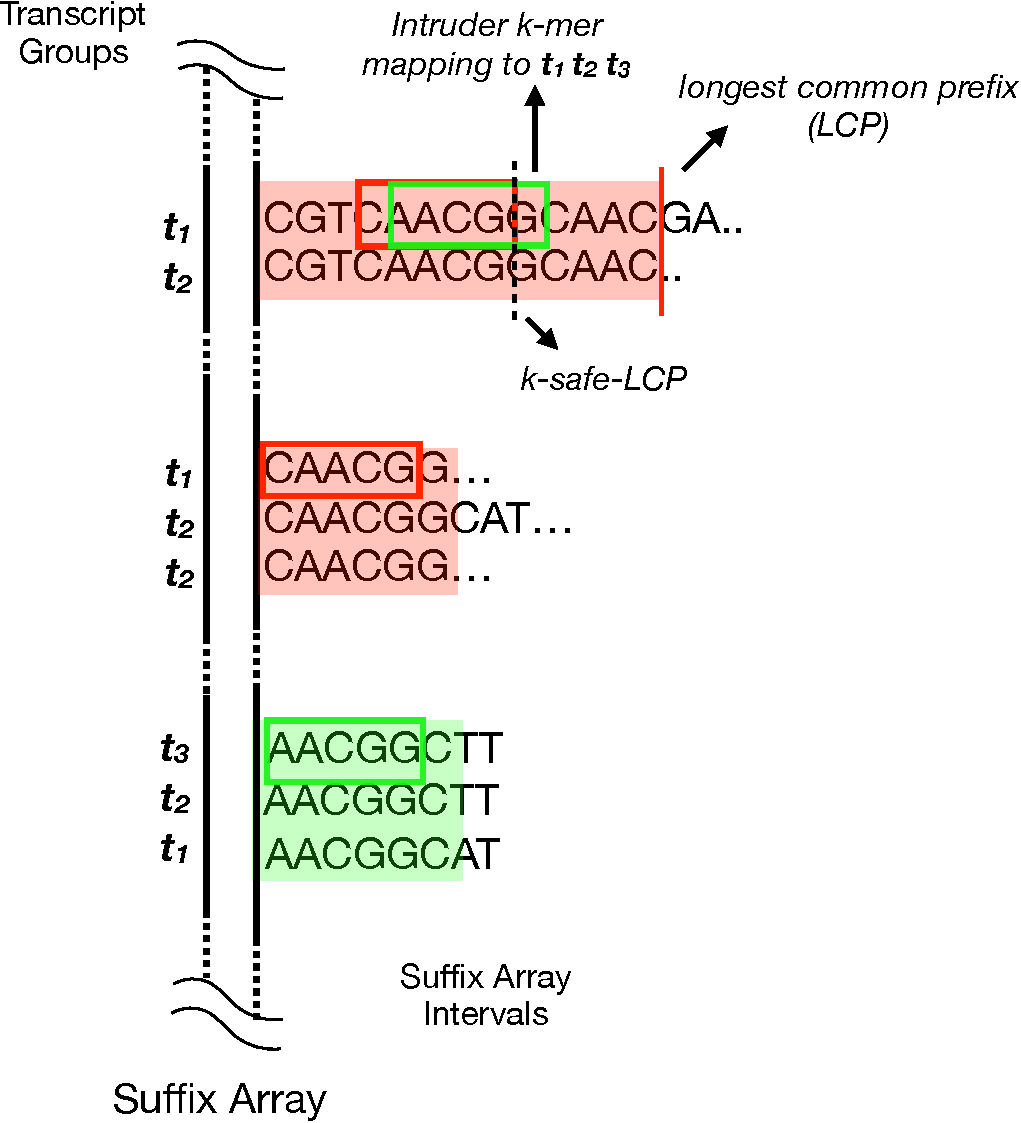
\includegraphics[scale=0.25]{Figures/sla/ksafelcp}
 \caption[Calculation of \kslcp from the suffix array data structure]
    {Calculation of \kslcp from the suffix array data structure. The
    transcripts present in each suffix array interval determine the relevant
    transcript sets, and which \kmers will be considered as intruders. To
    determine the \kslcp of the suffix array interval starting with the \kmer
    $CGTCA$, we check all the \kmers sequentially. Some \kmers do not yield an
    interval with transcripts other than $t_1$ and $t_2$, e.g., $CAACG$.
    Detection of a \kmer ($AACGG$) (as intruder) that maps to suffix array interval 
    labeled $(t_1,t_2,t_3)$ determines the \kslcp here.}
    \label{fig:safelength}
\end{figure}

\begin{figure}%[h]
 \centering
 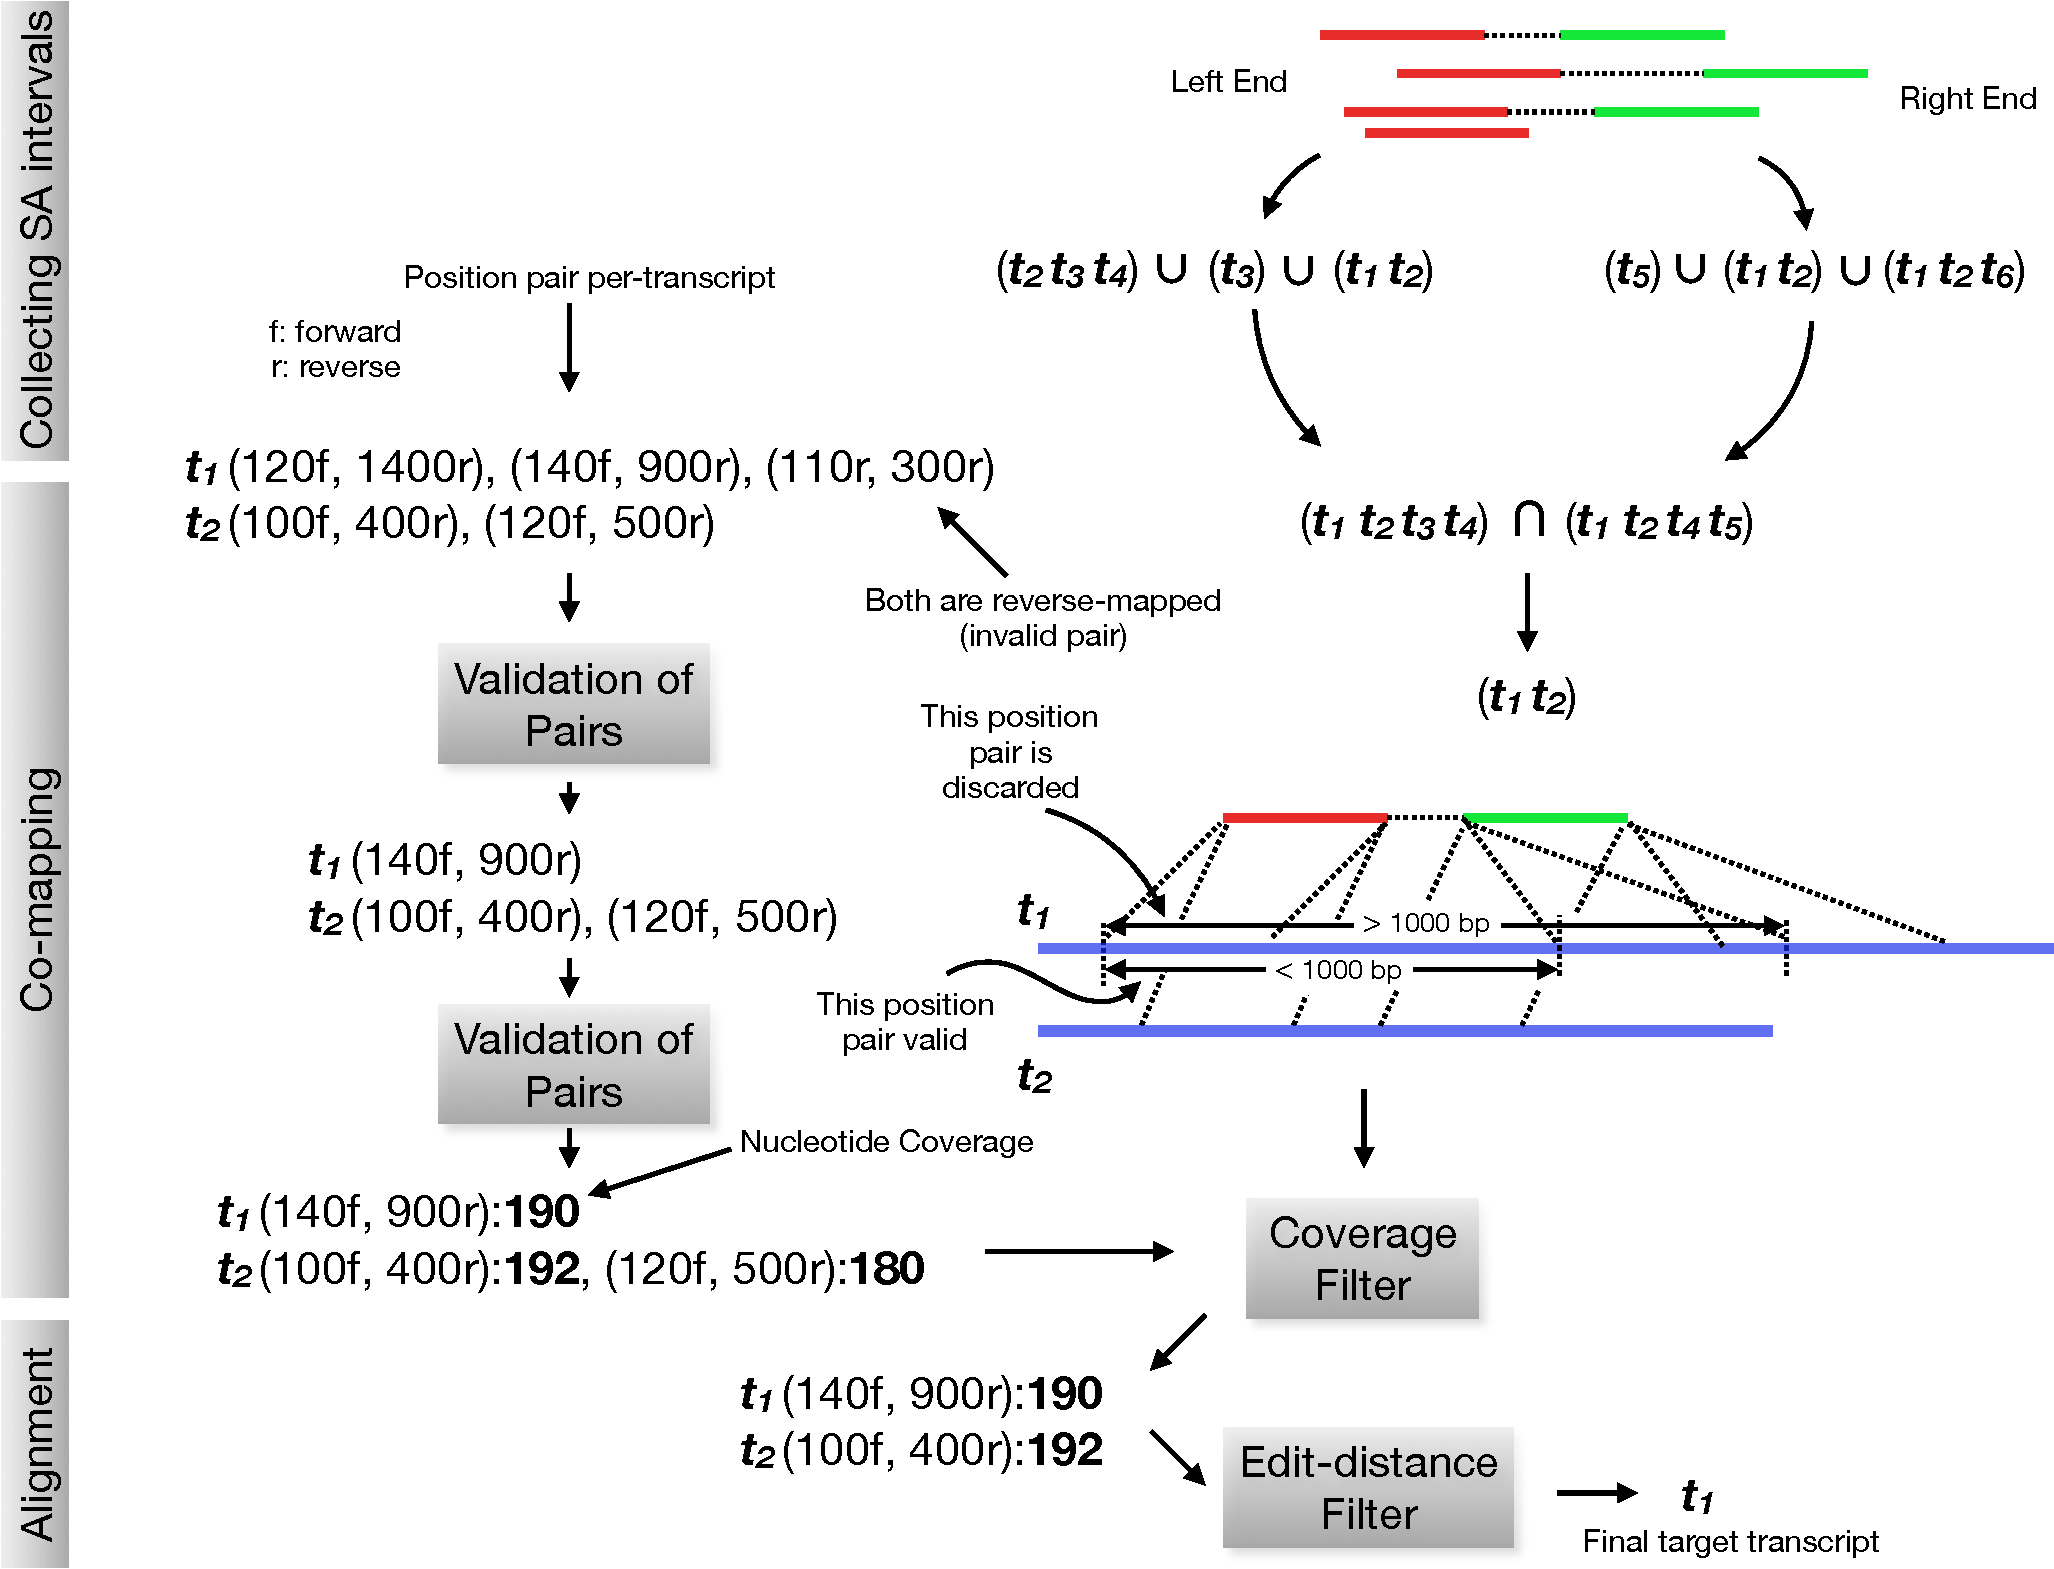
\includegraphics[scale=0.3]{Figures/sla/overview}
 \caption[The main steps of the \sla process]{The three main steps of the \sla 
 process are demonstrated here. First, suffix array ``hits'' are collected. Then, 
 in \cm, spurious mappings are removed by the orientation filter and then distance 
 filter. At most a single locus per-transcript is selected based on the coverage filter. 
 Finally, an edit-distance-based filter is used to select the valid target transcripts.
 }
  \label{fig:block_overview}
\end{figure}

\subsection{Defining and computing \kslcps}\label{sec:safelength}
Here, we formally define the concept of \kslcps (see figure~\cref{fig:safelength}). 
The determination of \kslcps starts by labeling each suffix array interval with the 
length of its corresponding longest common prefix and the associated transcript set it 
represents. Formally, $\LCP{\SuffixArray{[b]}}{\SuffixArray{[e-1]}}$ for an interval 
$\interval{b}{e}$ is the length of the common prefix of the suffixes $\SuffixArray{[b]}$ 
and $\SuffixArray{[e-1]}$. Given \kmer \samplekmer, where $\samplekmer \in \allkmers$ 
and \allkmers is the set of all \kmers from the reference sequence $T$, and the related 
interval $\ival{\samplekmer} = \interval{b}{e}$, for all $p \in \interval{b}{e}$, we 
consider each transcript $t$ such that the suffix $\SuffixArray{[p]}$ starts in transcript 
$t$ in the concatenated text. Then, for this interval, we can construct a set 
$\mathcal{C}^{\samplekmer} =  \{t_{i}, t_{j}, \dots\}$, which denotes the set of distinct 
transcripts that appear in the suffix array interval, indicated by \samplekmer.  We note 
that this notion discards duplicate appearances of the same transcript in this interval.

We compute the \kslcp for an interval indicated by \kmer $\samplekmer_i$ iteratively. The 
initial length for the \kslcp of the interval is $k$, length of a \kmer. We check, 
sequentially, each of the \kmers in the longest common prefix of the interval. For each 
new \kmer, the \kslcp is increased by one character. We terminate the \kslcp extension if 
any of the following conditions is encountered: (1) we reach the last \kmer contained 
in the LCP of this interval, (2) we encounter a \kmer $\samplekmer_j$ such that 
$\mathcal{C}^{\samplekmer_j} \not \subseteq \mathcal{C}^{\samplekmer_i}$ or (3) we 
encounter a \kmer $\samplekmer_j$ such that the reverse complement of $\samplekmer_j$ 
appears elsewhere in the transcriptome. When we encounter case (2) or (3), we call the 
\kmer $\samplekmer_j$ an \emph{intruder}.  That is, the \kmer will potentially alter our 
belief about the set of potential transcripts to which a sequence containing this \kmer 
maps (by strictly expanding this set), or the orientation with which it maps to the 
transcriptome.  We denote the \kslcp of a particular interval $\ival{\samplekmer_i}$ 
as $\mathrm{\texttt{\kslcp}}(\ival{\samplekmer_i})$.

As shown in figure~\cref{fig:safelength}, the \kslcp determination for the top suffix 
array interval starts with matching \kmers within the longest common prefix. The 
\kmer ``CAACG'' maps to a suffix array interval labeled with $(t_1,t_2)$. The next 
\kmer ``AACGG'', on the other hand, maps to a suffix array interval (shaded in green) 
labeled with $(t_1,t_2,t_3)$, thereby implying the \kslcp, shown as a dotted line. For 
each \kmer in the hash table, we store the length of the LCP and \kslcp, along with 
the corresponding suffix array interval.

\subsection{Discovering relevant suffix array intervals}
As shown in figure~\cref{fig:block_overview}, the selective-alignment approach can be 
broken into three major steps: collecting suffix array intervals, \cm, and selecting 
the high quality mappings. Gathering the suffix array intervals for a query read closely 
follows the \qm approach. It involves iterating over the read from left to right and 
repeating two steps. First, hashing a \kmer from the read sequence and then discovering the 
corresponding suffix array intervals. The process of \kmer lookup is aided by the \kslcp 
stored in the index (discussed in~\cref{sec:safelength}). The inbuilt lexicographic ordering 
of the suffixes in the suffix array, and the computed \kslcp values of intervals enable 
safely extending k-mers to longer matches without the possibility of masking 
potentially-informative substring matches. Given a matching \kmer, $\samplekmer_r$, 
from the read sequence $r$, we extend the match to find the longest substring of the 
read that matches within $\mathrm{\texttt{\kslcp}}(\ival{\samplekmer_r})$. The matched 
substring can be regarded as maximum mappable prefix (MMP)~\citep{Dobin2013Star}, that 
resides within the established \kslcp. We call this a maximal mappable safe prefix 
(MMSP --- eliding $k$ where implied). For a \kmer, $\samplekmer_r$, and interval, 
$\interval{b}{e}$, we note that $\mathrm{\texttt{\kslcp}}(\ival{\samplekmer_r}) 
\geq \length{\MMSP_{\samplekmer_r}}$, where $\length{\MMSP_{\samplekmer_r}}$ is the 
length of $\MMSP_{\samplekmer_r}$, the MMSP between the read's suffix starting with 
$\samplekmer_r$ and the interval $\ival{\samplekmer_r}$. The next \kmer lookup starts 
from the $(\MMSP_{\samplekmer_r}-k+1)$-th position. By restricting our match extensions 
to reside within the MMSP, we ensure that we will not neglect to query any k-mer that 
might \emph{expand} the set of potential transcripts where our read may map. We note 
here both the theoretical and practical relation between the \MMSP matching procedure, 
and the concept of a uni-MEM, as introduced by~\citet{debga}. The \kslcp for suffix array 
intervals are closely related to the lengths of unipaths in the reference de Bruijn 
graph of order $k$. Thus, our procedure for finding \MMSP{s}, that limits match 
extension by the \kslcp, is similar to the uni-MEM seed generation procedure described 
in debga \citep{debga}, with the distinction that in our method, we only consider extending 
seeds in one direction, and that we also choose not to terminate the \kslcp when the set 
of implied reference transcripts corresponding to the interval decreases in cardinality.

Given all the suffix array intervals collected for a read end (i.e. one end of a 
paired-end read), we take the \emph{union} of all the transcripts they encode. 
Formally, if  a read $r$ maps to suffix array intervals labeled with $\mathcal{C}^{r_1}, 
\ldots, \mathcal{C}^{r_n}$, then we consider all transcripts in the set $\mathcal{C}^{r_1} 
\cup \mathcal{C}^{r_2} \cup \ldots \cup \mathcal{C}^{r_n}$, and the associated positions 
implied by the suffix array intervals. As shown in~\cref{fig:block_overview}; 
this step is done before \cm.

We adopt a heuristic to avoid excessive \kmer lookups when we encounter a mismatch. 
When extension of an MMP is no longer possible, it is most probable that the mismatch 
results from an error in the read. If the mismatch is due to the presence of an error, 
then checking each \kmer overlapping this error can be a costly process. Instead, 
we move forward by a distance of $k/2$ in the read, and check the \kmer from the read 
such that the mismatch occurs in the middle position. If this \kmer lookup leads to 
another suffix array interval, we continue with the MMP extension process there; 
otherwise, we move again to the first \kmer that does not overlap this mismatch 
position. We observe that, in practice, the \kslcp, and hence the MMSP lengths can 
be quite large (\Cref{fig:dist}).

\subsection{Co-Mapping}
After collecting the suffix array intervals corresponding to left and right ends of the read, we wish to exploit 
the paired-end information in determining which potential mapping locations might be valid.  Hence, from this step 
onward, we use the joint information for determining the position and target transcripts. Given the suffix array 
intervals for individual ends of a paired-end read, the problem of aligning both ends poses a few challenges. 
First, a single read can map to multiple transcripts, and we wish to report all equally-best loci. Second, there 
can be multiple hits from a read on a single transcript (e.g., if a transcript contains repetitive sequence), and 
extra care must be taken to determine the correct mapping location. Finally, there may be hits that do not yield 
high-quality alignments (i.e. long exact matches that are nonetheless spurious).  To address the first and third 
points, we employ an edit distance filter to discard spurious and sub-optimal alignments.  To address the second 
challenge, we devise a consensus strategy to choose at most one unique position from each transcript.

Before applying the above mentioned strategy, we remove transcripts that do not contain hits from both the left 
and right ends of the read. Formally, given two ends of a read $r$, $r^{e_1}$ and $r^{e_2}$, and the corresponding 
suffix array intervals labeled with $\mathcal{C}^{r_1^{e_1}}, \ldots, \mathcal{C}^{r_n^{e_1}}$ and 
$\mathcal{C}^{r_1^{e_2}}, \ldots, \mathcal{C}^{r_m^{e_2}}$ respectively, we only consider transcripts present in 
the set $(\mathcal{C}^{r_1^{e_1}} \cup \ldots \cup \mathcal{C}^{r_n^{e_1}}) \cap (\mathcal{C}^{r_1^{e_2}} 
\cup \ldots \cup \mathcal{C}^{r_m^{e_2}})$.
We further refine this set by checking the validity of the alignments these hits might support. Currently, 
we use two validity checks illustrated in~\cref{fig:block_overview}. First, we apply an orientation-based 
check, and second, we employ a distance-based check. The orientation check removes potential mappings which have 
an orientation inconsistent with the underlying sequencing library type (e.g., both ends of a read mapping in the 
same orientation). The distance check removes potential alignments where the implied distance between the read 
ends is larger than a given, user-defined threshold ($1,000$ nucleotides by default).

\begin{figure}
 \centering
 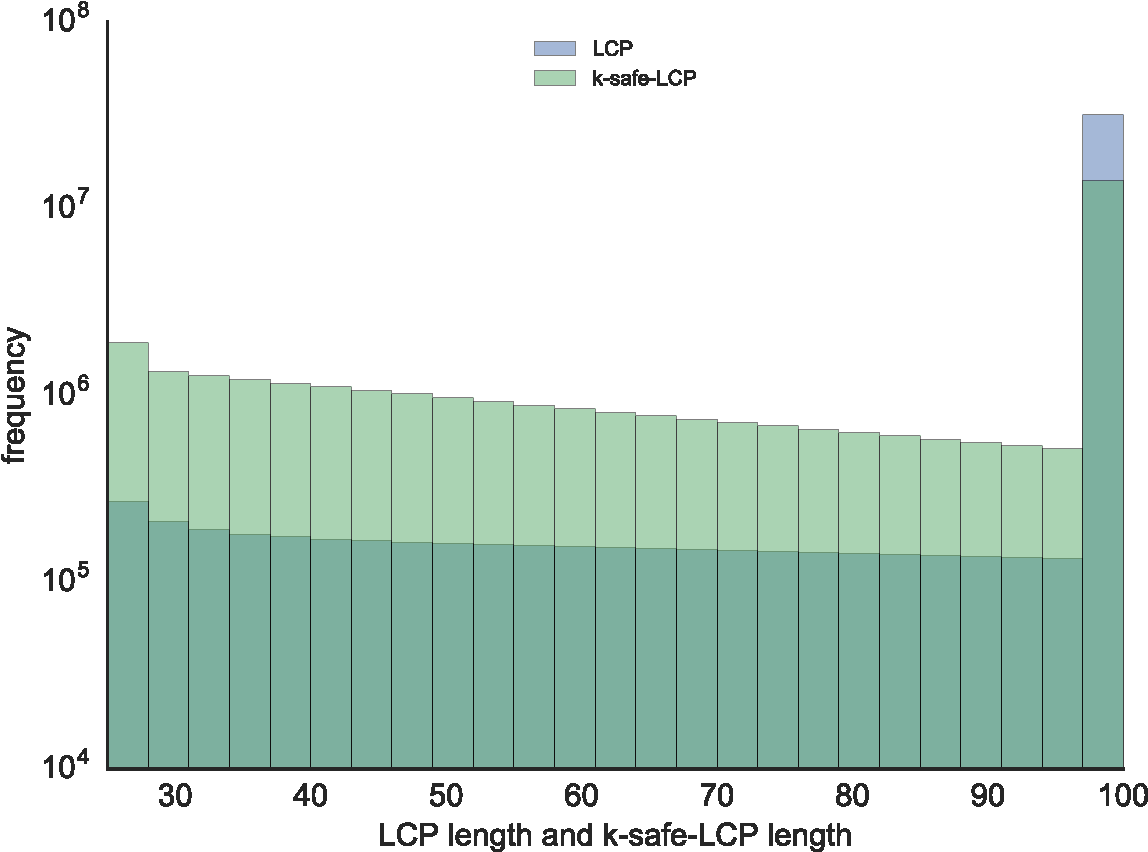
\includegraphics[scale=0.40]{Figures/sla/dist_safelength-color}
 \caption[The distribution of \kslcp lengths and LCP lengths]{The distribution of \kslcp lengths and LCP lengths 
 are similar and tend to be large in practice (human transcriptome).  Here, we truncate all lengths to a maximum 
 value of 100 (so that any LCP or \kslcp longer than 100 nucleotides is placed in the length 100 bin).}
\label{fig:dist}
\end{figure}

\begin{figure}
 \centering
 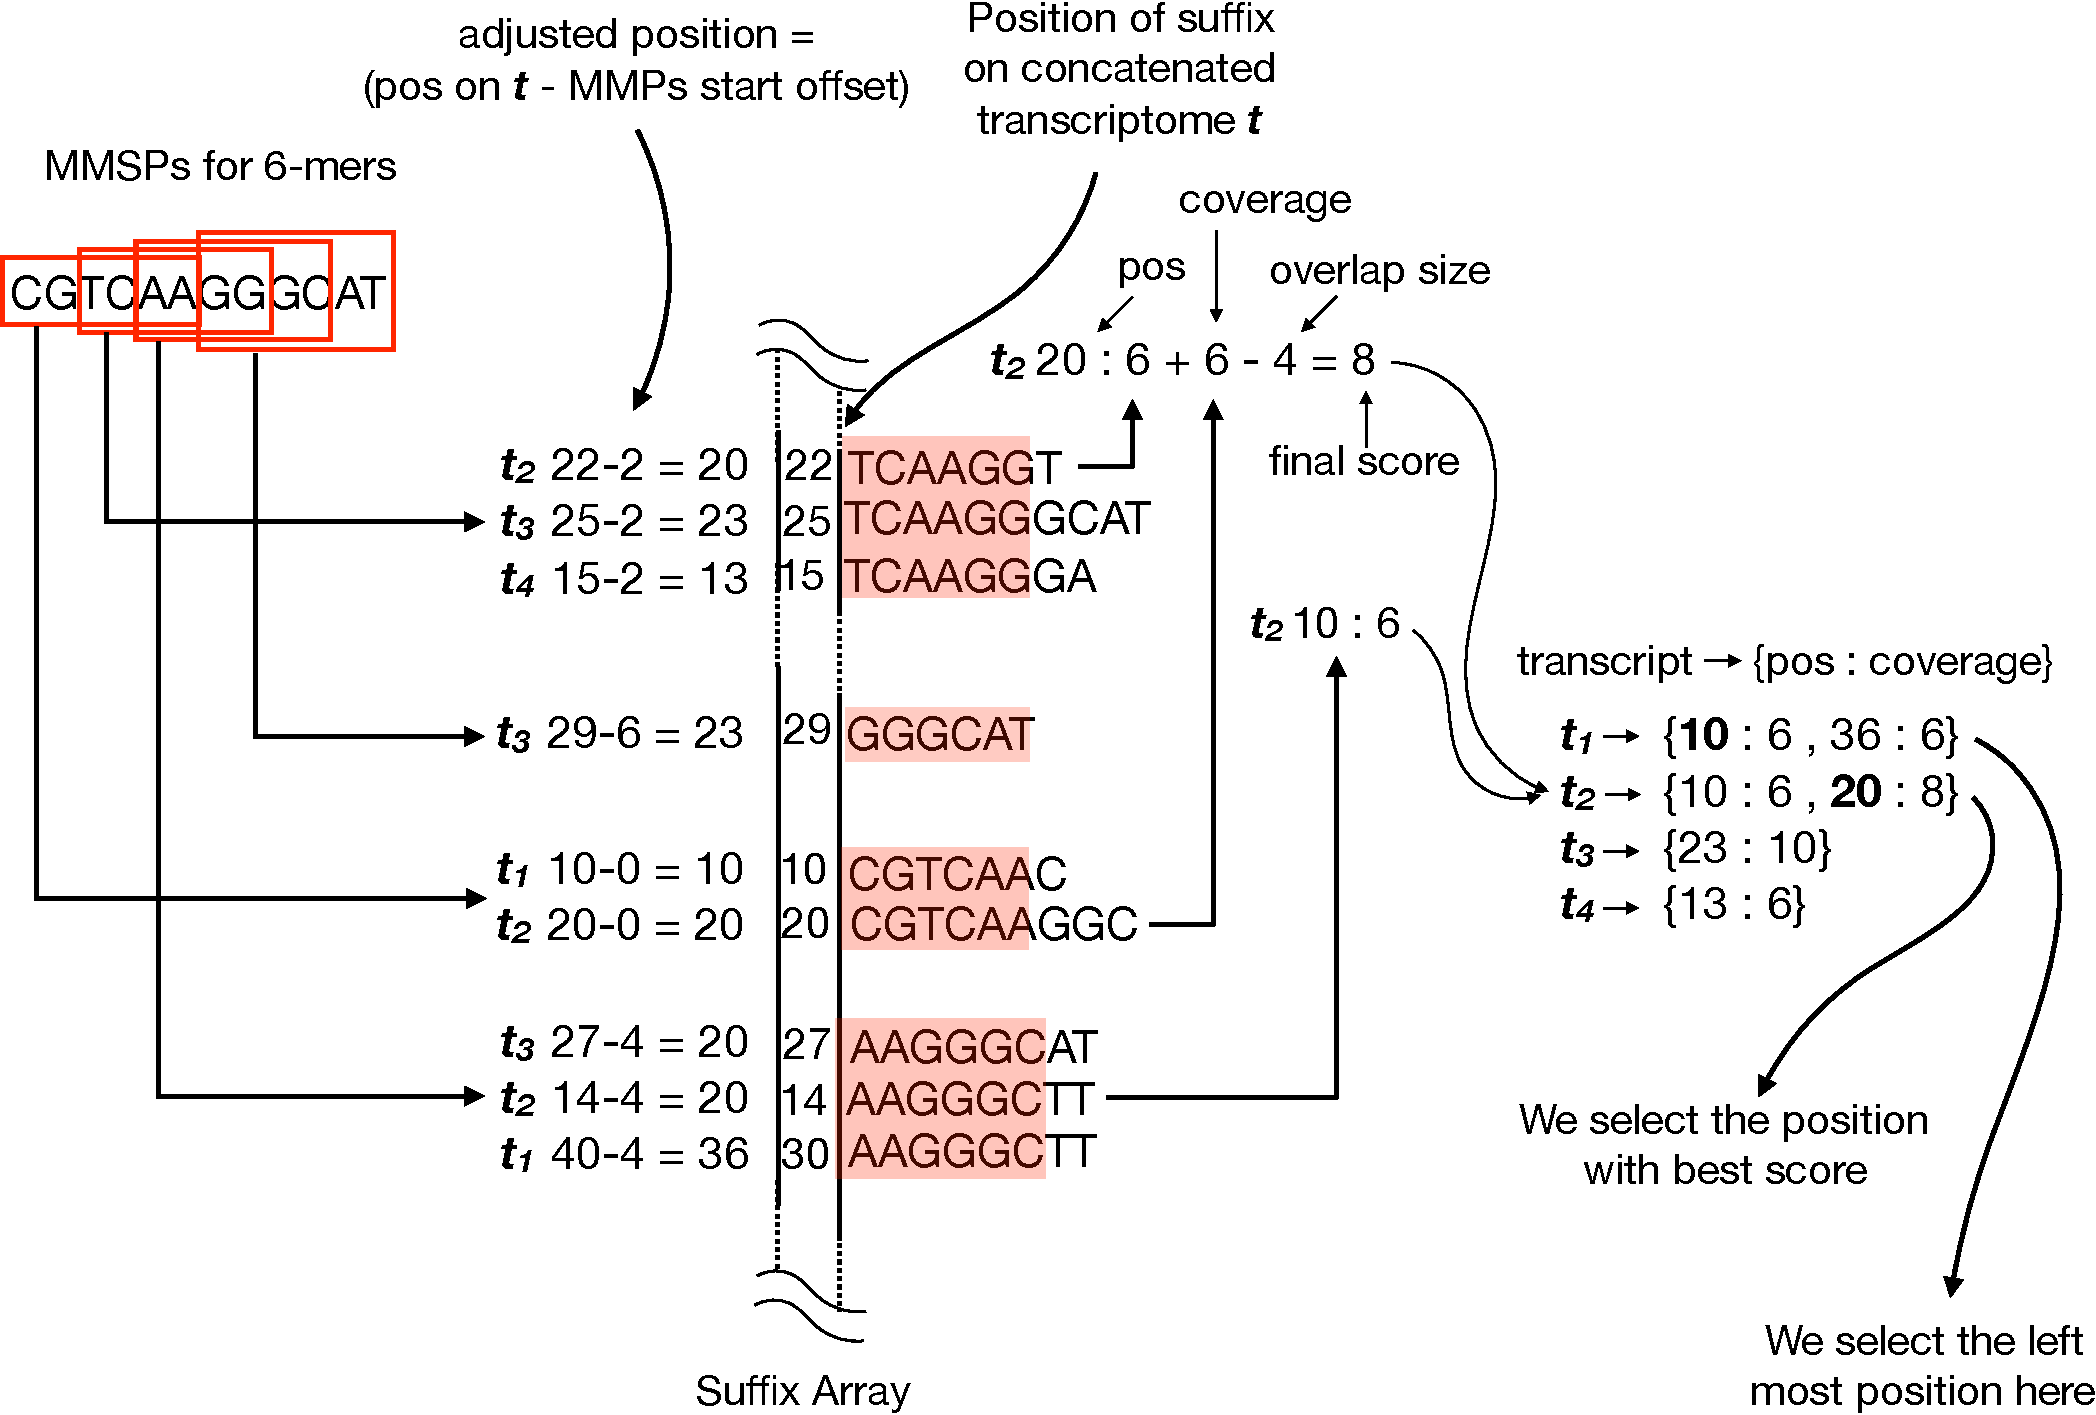
\includegraphics[scale=0.25]{Figures/sla/max_cov-color}
 \caption[Choosing the best postion on a transcript from multiple candidates]{The MMSPs corresponding to a read 
 are derived from multiple suffix array intervals. Here, all MMSPs happen to be of length $k$ as LCPs are of 
 size $k$. The coverage scheme finds out the exact positions on each transcript by adjusting the starting position of the MMSPs. The total score takes into account the positions where matches overlap. The final position is chosen by selecting the locus with maximum coverage.}
\label{fig:maxCov}
\end{figure}

\paragraph{Coverage based consensus:}
In \sla, the potential positions on a transcript are scored by their individual coverage on the target transcript.~\Cref{fig:maxCov} depicts the mechanism of choosing the best postion on a transcript from multiple probable mappings to the same transcript. The coverage mechanism employed in \sla makes use of the MMSP lengths collected during a prior step of the algorithm rather than simply counting \kmers. In~\cref{fig:maxCov}, the transcript $t_2$ has two potential mapping positions given the reads: position 10 and 20. The coverage consensus mechanism selects position 20 over position 10 due to the higher coverage by tiling MMSPs on the read.

\subsection{Selecting the best candidate transcripts}
Once the positional ambiguity within a transcript is resolved, the next step is selecting the best candidate transcripts from a set of mappings. Since mapping relies on finding exact matches, the length of the matched subsequence between the read and reference can sometimes be misguiding when comparing different candidate transcripts. That is, the transcripts with the longest exact matches do not always su A block diagram of the steps described below are depicted in Figure pport optimal alignments for a read.  At this point in our procedure, we follow the approach taken by many conventional aligners, and use an existing optimal alignment algorithm to compute the edit distance, by which we select the best candidate transcripts.

When performing alignment, we assume that a given read aligns starting at the position computed in the previous steps.  This helps us to reduce the search space within the transcript where we must consider aligning the read, and thereby considerably reduces the cost of alignment. To align the read at a specific position on the transcript and calculate the edit distance between them, we use $Myer's$ bounded edit distance bit-vector algorithm~\citep{myers1999fast}, as implemented in \texttt{edlib}~\citep{edlib}.  For a fixed maximum allowable edit distance, this algorithm is linear in the length of the read. We note that the bounded edit distance algorithm we employ will automatically terminate an alignment when the required edit distance bound is not achievable.

We remove all alignments with edit distance greater than a user-provided threshold. This is similar to the approach used by many existing aligners, and allows us to specify that even the best mapping for a given read may have too many edits to believe that it reasonably originated from a known transcript in the index. An appropriate threshold should be based on the expected error rate of the instrument generating the sequenced reads, and a very low threshold can lead to a decreased mapping rate.

\subsection{Enhancement of quantification accuracy based on edit distance}\label{filter}
We investigated the effect of incorporating edit distance in downstream quantification. Since we integrated the \sla scheme into the quantification tool \salmon \citep{Patro2017Salmon}, the edit distance scores from \sla can be used as a new parameter to \salmon{}'s inference algorithm.

%\mohsen{I modified some notations in the following paragraph, please verify if every thing is sound.}
In the framework of abundance estimation, we define the conditional probability of a generating a particular fragment, $f_j$, given that it comes from a specific transcript, $t_i$, as $P(f_j \mid t_i)$. Given the edit distance between the fragment and the transcript, we can incorporate this parameter into this conditional probability. \emph{Soft} filtering introduces a new term in the conditional probability based on $d_{i,j}$, which is the sum of the edit distances between the read ends of fragment $f_j$ and transcript $t_i$. We set this probability according to an exponential function, $P(a_{j}|f_j,t_i)=e^{-4d_{i,j}}$. The aggregate of threshold filtering and \emph{soft} filtering can be described as follows:\\

\begin{equation}
\Pr\left( a_{j} \mid d_{i,j}, \txp{i} \right)  =
      \begin{cases}
      0  & \text{$d_{i,j} > threshold$}\\
      e^{-4d_{i,j}}  &\text{$d_{i,j} \le threshold$}
      \end{cases}.
  \label{eqn:softFilter}
\end{equation}

\paragraph{Preventing redundant alignments by exploiting shared LCPs:}\label{sharedLCP}
Exploiting the common subsequences in the transcriptome is instrumental to the superior speed of fast mapping, 
\nab tools. Reads generated from exonic sequences common to multiple transcripts from the same gene or paralogous 
genes are the main source of ambiguous mappings. As we rely on the suffix array data structure to obtain the 
initial set of transcripts to which a read maps, there are cases where exactly identical reference sequences 
all act as mapping targets for the read. For a suffix array interval $\interval{b}{e}$, we identify such common 
subsequences by examining the {\it longest common prefix} (LCP) of the interval. If the length of the LCP is 
equal or greater than the length of the read, then the actual alignment against the underlying reference at 
these positions will be identical. We observed that for almost half of the read-transcript pairs, the alignment 
process can be avoided. Note that if the read sequence shares a complete match with the common prefix, meaning 
that maximum mappable safe prefix length is equal to read length (i.e., the read matches the reference exactly 
at some set of positions), we can also bypass the Meyer's edit distance algorithm call completely.

\paragraph{Avoids redundant work by caching alignment sub-problems further:} We also extend a similar idea to the 
scenario where only part of the reference sequence is shared between references.  Specifically, when performing an 
alignment between anchoring exact matches, we store the result in a hash table where the key is a tuple 
$\left(i,j,h\left(i', j'\right)\right)$ and the associated value is the computed edit distance.  Here, $i$ 
and $j$ denote the start and end of the read interval being aligned and $i'$ and $j'$ denote the start and 
end of the reference sequence; $h(i',j')$ is a hash of the corresponding reference sequence 
(we use \texttt{xxhash}~\citep{xxhash}).  This allows us to detect when a redundant alignment sub-problem for 
a read is shared between references, and to reuse the cached result in such cases.


\subsection{Evaluating the performance of \sla}


To evaluate the effectiveness of \sla, we coupled it with the quantification tool \salmon (branching from the v0.9.1 
release). This enables us to measure the effect of different alignment based and non-alignment based algorithms on 
transcript-level quantification results directly, holding the statistical estimation procedure fixed. We also include 
\kallisto(v0.43) in our benchmarks, which provides a perspective on \pa-based quantification. Furthermore, we compare 
the performance of \sla with the recent, fast, hashing and alignemnt-based, abundance estimation tool (currently un-published) 
\hera~\footnote{\url{https://github.com/bioturing/hera}}. We note, this is an early version of the \hera(v1.2) software, 
which is already performing very well in our testing, but is subject to changes and improvements. Given it's impressive 
performance (in both time and accuracy), we decided to include \hera in our comparisons with the consent of its authors 
(personal communications). We measure the Spearman correlation and Mean Absolute Relative Differences (MARD) of read 
counts as performance metrics when comparing the different methods.
%(further metrics are also provided for some of the experiments in the supplementary material). 
All experiments of this section were performed on an Intel(R) Xeon(R) CPU (E5-2699 v4 @2.20GHz 
with 44 cores and 56MB L3 cache) with 512GB RAM and a 4TB TOSHIBA MG03ACA4 ATA HDD running ubuntu 16.10 and each method 
was run using 16 threads.

In all our experiments, reads are mapped to the transcriptome using using \bt, \kallisto, \hera, \sla and \STAR. 
Subsequently, transcripts are quantified by \salmon(v0.9.1) using the relevant mappings (from alignment or the 
\nab methods) as input (except in the cases of \kallisto(0.43) and \hera(1.2), which include implementations of 
their quantification algorithms). The alignment mode of \salmon enables us to use \STAR(v2.5) and \bt(v2.3) output 
as a direct input to the quantification module --- thereby reducing variability due to differences in the 
underlying methodology used for quantification. To achieve the most sensitive alignment, \bt is run with the 
alignment options suggested for use with \rsem~\citep{rsembmc}. For aligning reads to the transcriptome using 
\STAR, we used the same options described in \citep{Srivastava2016rapmap}. When processing alignments, \salmon 
was run with \texttt{-{}-rangeFactorizationBins 4}~\citep{ismb2017factorization} and \texttt{-{}-useErrorModel}. 
With \sla, \salmon was run using the \texttt{-{}-softFilter} flag (discussed in~\cref{filter}), 
a range factorization value of 4 and an edit distance threshold of 7. \kallisto was run with default parameters. 
Both the \sla and \kallisto indices were built with $k=25$; \hera does not include \kmer size as a user-defined 
parameter.

\subsection{Quantification of simulated reads against mutated transcriptomes}\label{subsec:synthetic}

We explored the performance of different alignment-based and alignment-free methods by quantifying simulated short 
RNA-seq reads against mutated reference sequences. The simulation process consists of two steps. In the first step, 
we mapped an experimental RNA-seq sample (accession number SRR5638585) to the human transcriptome (Ensembl release 
80 \citep{yates2015ensembl} ) using \salmon. The resulting abundance vector, in conjunction with the full 
transcriptome sequence generated from the full human genome and the corresponding annotations (version GRCh37.p13), 
is used to simulate five batches of 100bp paired-end RNA-seq samples, where each batch contains $\sim47$M reads. 
We used the sequence simulator Polyester \citep{frazee2015polyester} for generating the read datasets.

While the simulated dataset enables comparison with the ground truth, the quality of the reads is high and does 
not show the subtle nuances that arise when mapping reads from experimental sequencing datasets. In reality, the 
sequenced reads could differ from the annotated reference sequence due the presence of mutations (variants) in the 
sequenced organism. In other cases, a reference sequence from one species could be used to analyze data from a 
phylogenetically closely related species, for which an annotated reference in unavailable. Therefore, to 
recapitulate these adversarial situations, instead of mapping the simulated reads to the exact underlying 
transcriptome used for read generation, we map them against references mutated at a controllable rate.

The mutated version of the transcriptome is derived from the underlying reference genome that was subject to 
random mutations. The nucleotides of the reference genome were randomly altered based on a Poisson process with 
a tunable {\it rate} parameter. The rate parameter enables controling the rate of mutation that we want to 
introduce in the reference genome. For the current manuscript we have used $5$ equally spaced rate parameters 
from $0.01$ to $0.05$. The mutated genome sequences and the original annotation are used to generate the mutated 
reference transcriptomes. As the resulting transcriptomes contain devations from the indexed reference, we believe 
that mapping to these references will capture some aspects of the difficulties encountered when applying such tools 
to certain experimental datasets.

To evaluate the performance we have measured the quantification accuracy of different tools with respect to the 
ground truth provided to Polyester. As explained earlier, tools such as \kallisto, \hera and \sla have a 
quantification pipeline attached to the mapping module and are, therefore, capable of generating abundance 
vectors directly. On the other hand, \bt and \STAR generate alignment files that we have coupled with \salmon 
(run in alignment-based mode) to obtain abundance estimates.

\begin{figure}
 \centering
 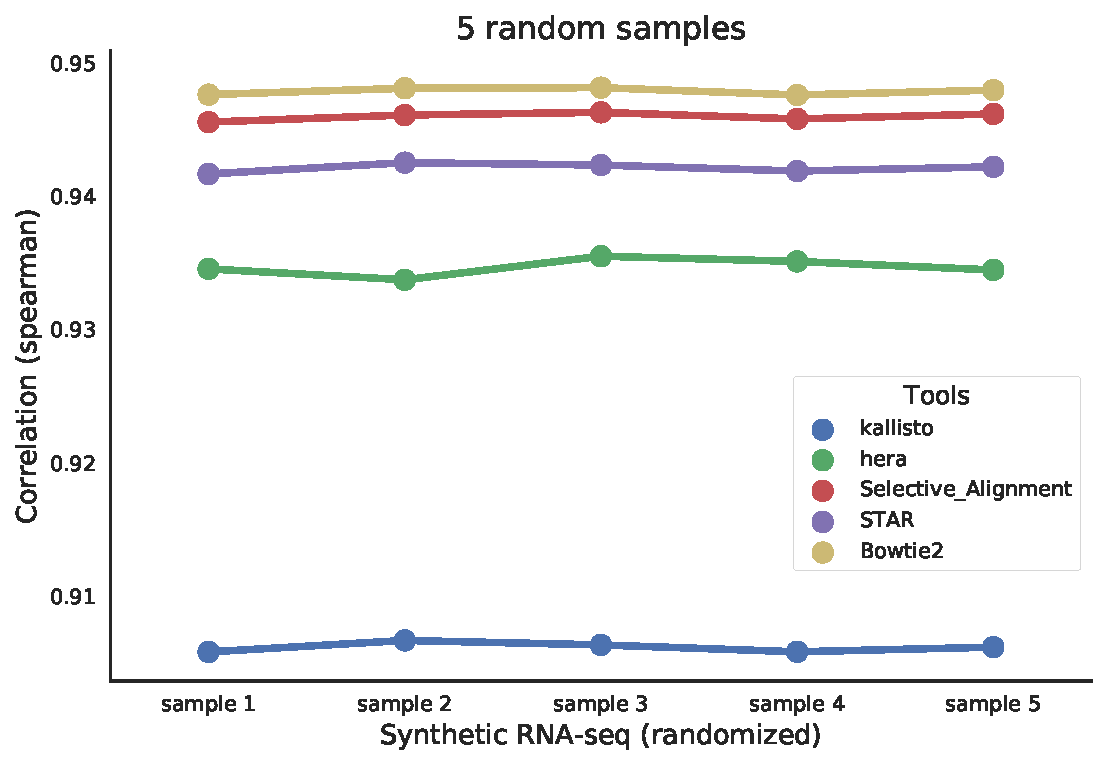
\includegraphics[scale=0.40]{Figures/sla/standard_error}
 \caption[Performance of tools on paired end reads]{Performance variation of 
 different tools on paired end reads produced with five random seeds.}
  \label{fig:random_samples}
\end{figure}

Performance of the various methods on a simulated sample is shown in~\cref{tab:diff_mutation_sp}
and~\cref{tab:diff_mutation_mard}. In this case, 
the simulated sample is mapped against $5$ different mutated transcriptomes with increasing error rates and the 
corresponding spearman correlation and MARD values calculated using the ground truth. As shown in 
\cref{tab:diff_mutation_sp}, the correlation between quantification estimates using \sla and the ground truth is 
higher than the other self-contained quantification methods, \kallisto and \hera. This gap between correlation 
values increases as the rate of mutation in the reference transcriptome is increased, showing the ability of 
\sla to accurately map reads against diverging transcriptomes. The MARD values for \sla are lower in comparison 
with other \nab methods as well.

To measure the variation in quantification about a single random instance of simulated data (i.e., data generated 
with a particular random seed), we have also generated five different simulated RNA-seq datasets by passing 
different seeds to Polyester. To minimize external variation, we used the least mutated transcriptome 
(rate 0.01) as reference. By plotting the spearman correlations, as shown in~\cref{fig:random_samples}, 
we observe that, given that all the tools perform well on the random samples, the performance of \sla is grouped 
with the alignment-based methods, such as \bt and \STAR.  Further, the variation in quantification performance of 
all methods (i.e. the standared error) across these different simulated replicates is very small.

\begin{table}
\begin{center}
\begin{tabular} {c|c c c c c}
\toprule
  Mutation Rate & Kallisto & Hera & Selective Alignment & STAR-Salmon &Bowtie2-Salmon \\
\midrule
  0.01 & 0.906 & 0.935 & \textbf{0.946} & 0.942 & \textbf{0.948} \\
  0.02 & 0.871 & 0.925 & \textbf{0.942} & 0.939 & \textbf{0.945} \\
  0.03 & 0.844 & 0.910 & \textbf{0.935} & 0.933 & \textbf{0.942} \\
  0.04 & 0.817 & 0.880 & \textbf{0.925} & \textbf{0.925} & \textbf{0.937} \\
  0.05 & 0.793 & 0.845 & 0.904 & 0.909 & \textbf{0.927} \\
\bottomrule
\end{tabular}
\caption[Acuracy of qunatification of synthetic dataset against the mutated reference transcriptome]{
  {Synthetic dataset quantified against the mutated reference transcriptome with different mutation rates. 
  The spearman correlation is calculated with respect to the ground truth.}
}
\vspace{-0.3in}
\label{tab:diff_mutation_sp}
\end{center}
\end{table}

\begin{table}
\begin{center}
\begin{tabular} {c|c c c c c}
\toprule
Mutation Rate & Kallisto & Hera & Selective Alignment & STAR-Salmon &Bowtie2-Salmon \\
\midrule
  0.01 & 0.161 & 0.116 & \textbf{0.100} & 0.104 & \textbf{0.096}\\
  0.02 & 0.193 & 0.132 & 0.108 & 0.109 & \textbf{0.100}\\
  0.03 & 0.215 & 0.172 & 0.120 & 0.115 & \textbf{0.107}\\
  0.04 & 0.236 & 0.231 & 0.143 & 0.127 & \textbf{0.118}\\
  0.05 & 0.257 & 0.291 & 0.186 & 0.150 & \textbf{0.142}\\
\bottomrule
\end{tabular}
\caption[MARD of qunatification of synthetic dataset against the mutated reference transcriptome]{
  {Synthetic dataset quantified against the mutated reference transcriptome with different mutation rates. 
  The MARD (mean absolute relative difference) is calculated with respect to the ground truth.}
}
\vspace{-0.3in}
\label{tab:diff_mutation_mard}
\end{center}
\end{table}


\subsection{Experimental reads from human transcriptome}\label{res:experimental}

We have also benchmarked our proposed \sla method on experimental data from SEQC(MAQC-III) 
consortium ~\citep{seqc2014comprehensive} samples (SRA accession \texttt{SRR1215996} - \texttt{SRR1216000}). 
Each of the five technical replicates consists of $\sim$11M$, 100$bp, paired-end reads, sequenced on an 
Illumina Hiseq 2000 platform.

We follow the same basic assessment methodology as discussed in~\cref{subsec:synthetic}, and report the mean 
Spearman correlation and MARD value for each method. However, we note that, since this is experimentally-derived 
data, there is no knowledge of ground truth transcript abundances.  Instead, we have measured the overall 
concordance between different approaches. Given the results obtained in all of our other testing, we expect 
the \bt-based pipeline to be the most accurate, so we are generally looking for high concordance with those 
quantifiaction estimates.

In~\cref{tab:correlations}, we compare the quantification results produced by different methods. Each 
individual cell contains the average obtained across the five samples. High Spearman correlation and low MARD 
value between \bt and \sla show that \sla produces results most similar to those based on \bt. Interestingly, 
the concordance between the \sla and \bt-based pipelines is even higher than the concordance between the two 
pipelines based on more traditional alignment approaches (i.e. \bt and STAR). While we cannot assess the accuracy 
with respect to known ground truth on these samples, we nonetheless believe assessments based on real data like 
this are important to perform, as the complexity of experimental data seems to be considerably higher than that 
of simulated data and its characteristics can be markedly different. Finally, \Cref{tab:experimental_timing} 
provides timing and memory assessments of all the methods running on sample \texttt{SRR1215996}. Since the 
mapping phase of \sla is not distinct from the quantification phase, the memory and time footprints include 
the mapping part of the pipeline.  Further, disk space is not comparable to alignment-based methods, since 
alignment files are not written directly as output of \sla (rather, the \sla algorithm informs the mappings 
and provides edit-distance-based scores --- as described in~\cref{eqn:softFilter} --- directly to the 
quantification algorithm).

\begin{table}
\renewrobustcmd{\bfseries}{\fontseries{b}\selectfont}
\sisetup{detect-weight,mode=text,group-minimum-digits = 4}
\centering
\begin{tabular}{|l|c|c|c|c|c|}
\hline
 Method & \kallisto &\hera  & selective & \STAR & \bt \\ %& \qm
\hline
\kallisto &  \diagbox[]{\num{1}}{\num{0}} & \num{0.189293544242057} 
& \num{0.160148930794467} & \num{0.152536064490726} & \num{0.168211319115239} \\
\hline
\hera & \num{0.868172058407572} & \diagbox[]{\num{1}}{\num{0}} 
& \num{0.134994519090086} & \num{0.147176566236675} & \num{0.137529630659189}\\
\hline
\ssla & \num{0.898126618322603} & \num{0.902170309453134} & \diagbox[]{\num{1}}{\num{0}} 
& \num{0.128558965365635}   & \ubold \num{0.0585736425878761}\\
\hline
\STAR &   \num{0.898360010715753} & \num{0.89565317161376} & \num{0.912909527305415} 
& \diagbox[]{\num{1}}{\num{0}} & \num{0.128710771202473} \\
\hline
\bt & \num{0.890488189578628} & \num{0.900958882919405} & \ubold \num{0.966015219762142} 
& \num{0.913252923042169} & \diagbox[]{\num{1}}{\num{0}} \\   \hline
\end{tabular}
\caption[The accuracy of quantifications computed by all methods on experimental data]
{The Spearman correlation and MARDS between transcript abundances computed by all methods on 
experimental data. Each number is the mean on 5 different samples; the numbers in the lower 
left triangle of the matrix are the Spearman correlations and the ones in upper right are 
the MARD values. "\ssla" refers to \sla.}
\label{tab:correlations}
\end{table}

\begin{table}%[h]
\centering
\begin{tabular}{lrr}
\toprule
Method &time (s) & memory (KB) \\
\midrule
\kallisto & \num{61} & \num{4006284} \\
\hera  & \ubold \num{38} & \num{6736576} \\
\sla & \num{65} & \num{7994324} \\
\STAR & 398+96 & max(\num{8342444},\num{5513432}) \\
\bt & 977+125 & max(\num{1020032},\num{9949380}) \\

\bottomrule
\end{tabular}
\caption[Comparison of timing and memory foot-print of \sla with other alignment and non-alignment methods]
{Comparison of timing and memory foot-print of \sla with other alignment and non-alignment methods 
on experimental sample SRR1215996. The timing performance for \STAR and \bt is the sum of mapping 
and quantification (with salmon) steps (first number is the mapping step) and memory footprint is 
the max memory footprint of these two steps (first number is for the mapping step).\\}
\label{tab:experimental_timing}
\end{table}

\subsection{Conclusion}
Recently, fast \nab approaches have been developed for mapping RNA-seq reads to transcriptomes. Rather than 
generating full alignments, these approaches compute ``mapping'' information that is often sufficient for 
a number of  given analysis tasks (e.g., transcript 
quantification~\citep{Patro2014Sailfish,zhang2014rna,Bray2016Kallisto,Patro2017Salmon,ju2017fleximer} 
or metagenomic abundance estimation~\citep{Schaeffer2017}). Yet, there exist scenarios where such \nab approaches 
can go awry; either failing, by the greedy nature of their procedures, to find the true target of origin of 
a read, or by allowing spurious mappings to targets supported by exact matches that would nonetheless fail 
reasonable alignment scoring filters. Moreover, it is sometimes desirable to be able to produce, on demand, 
the edit distance or alignment that would result from a given mapping location. The recently-introduced \hera 
validates mapping quality using alignment, which resolves spurious mappings, though it still suffers a loss of 
sensitivity compared to traditional alignment methods, and fails to process \denovo assembled transcriptomes. 
In this section, we introduced a selective alignment algorithm that attempts to bridge the gap between these \nab 
algorithms and more traditional alignment approaches. \Sla improves upon both the sensitivity and specificity 
of these \nab algorithms while making very moderate concessions with respect to the computational budget. 
To achieve this level of efficiency, a number of algorithmic innovations were required, some of which may be of 
general interest. In the future, we hope to expand upon the notion of selective alignment even further, both by 
improving the algorithm and implementation, and by exploring use cases where selective alignment applies. Such 
situations are those where fast \nab approaches are inappropriate and traditional alignment approaches are too 
slow. In terms of improving the method, we hope to add functionality to automatically predict the optimal edit 
distance threshold in the read mappings based on the quality of the alignments, and for \sla to self-tune to 
properly handle edge cases, such as soft clipping. The \sla algorithm currently implements user specified edit 
distance threshold for filtering spurious reads. A more data-driven choice of filter can lead to a more resilient 
threshold that can perform gracefully while handling both adversarial reads as well as high-quality reads in 
heterogeneous read samples. In high quality samples, the edit distance bound can be set lower to further 
speed-up the algorithm. Future work will also include support for reporting the actual CIGAR strings for 
applications that require this information, such as RNA-seq based variant calling or allele identification.

\section[Puffaligner]{Puffaligner: An efficient and accurate aligner based on the pufferfish index}
Short-read aligners are a major workhorse of modern genomics. Given the importance of the alignment problem, 
a tremendous number of different tools have been developed to tackle this problem. Some widely used examples are
\bwa~\citep{bwa}, \bt~\citep{bowtie2}, \hisat~\citep{hisat,hisat2} and \st~\citep{star}.
Existing alignment tools use a variety of indexing methods. Some tools, such as \bwa, \bt, and \st
use a full-text index over the reference sequences; \bwa and \bt use variants of the FM-index, 
while \st uses a suffix array.

A popular alternative approach to full-text indices is to instead, index sub-strings of length $k$ (\kmers) 
from the reference sequence. Trading off index size for potential sensitivity, such indices can either index
all of the \kmers present in the underlying reference, or some uniform or intelligently-chosen sampling of \kmers. 
There are a large variety of \kmer-based aligners, including tools like the Subread
aligner~\citep{subread}, SHRiMP2~\citep{shrimp2}, mrfast~\citep{mrfast}, and mrsfast~\citep{mrsfast}. 
To reduce the index size, one can choose  to select specific \kmers based on a winnowing (or minimizer) scheme.
This approach has been particularly common in tools designed for long-read sequence alignment like 
mashmap~\citep{Jain2018} and minimap2~\citep{minimap2}.

Recently, a set of new indices for storing \kmers have been proposed based on graphs, specifically \dbgs (\dbgshort). 
A \dbg is a graph over a set of distinct \kmers where each edge connects two neighboring \kmers
that appear consequently in a reference sequence and therefore, overlap on ``$k-1$'' bases. \kallisto~\citep{kallisto}, 
\debga~\citep{debga}, BGreat~\citep{bgreat}, \brownie~\citep{brownie}, and \pufferfish~\citep{pufferfish} are some
tools which use an index constructed over the \dbg built from the reference sequences. 
Cortex~\citep{cortex}, Vari~\citep{vari}, rainbowfish~\citep{rainbowfish}, and mantis~\citep{mantis} are also tools
that use a \ccdbg for building their index over a set of raw experiments. All these approaches cover a wide range 
of the possible design space, and different design decisions yield different performance tradeoffs.

Generally, the fastest aligners (like \st) have very large memory requirements for indexing, and make 
some sacrifices in sensitivity to obtain their speed. On the other hand, the most sensitive aligners (like
\bt) have very moderate memory requirements, but obtain their sensitivity at the cost of a higher runtime. 
Maintaining the balance between time and memory is especially more critical while aligning 
to a large set of references, like a large collection of microbial  and viral genomes which may 
be used as an index in microbiome or metagenomic studies. As both the collection of reference genomes and 
the amount of sequencing data grows quickly, it is import for alignment tools to achieve a time-space balance 
without loosing sensitivity.

Based on the compact \pufferfish~\citep{pufferfish} index, we introduce a new aligner called \puffaligner,
that we believe strikes an interesting and useful balance in this design space. \puffaligner is designed 
to be a highly-sensitive alignment tool while, simultaneously, placing a premium on computational overhead.
By using the \ccdbg to factor out repeated sub-sequences in the reference, it is able to leverage the speed 
and cache friendliness of hash-table based aligners while still controlling 
the growth in the size of the index; especially in the context of redundant reference sequences. By carefully 
exploring the alignment challenges that arise in different assays, including single-organism DNA-seq, 
RNA-seq alignment to the transcriptome, and metagenomic sequencing, we have engineered a versatile
tool that strikes desirable balance between accuracy, memory requirements and speed. We compare 
\puffaligner to some other popular aligners and show how it navigates these different tradeoffs. 
\puffaligner is a free and open-source software and it is implemented in C++14 and can be obtained 
from \url{https://github.com/COMBINE-lab/pufferfish/tree/cigar-strings}.

\subsection{Main pipeline in \puffaligner}
\puffaligner is an aligner built on top of the \pufferfish indexing data structure. \pufferfish is a 
space-efficient and fast index for the \ccdbg (\ccdbgshort). A \ccdbg is a graph whose vertices
(strings) are the compacted non-branching paths of the underlying \dbg, with the restriction that 
each node also have the same color set (set of reference sequences in which it appears). The nodes in the
\ccdbg are referred to as \unitigs. Each \unitig can be mapped to a list of $<$reference ID, position, 
orientation$>$ tuples that describe exactly how this subsequence appears in the unlderying
collection of references. The basic query operation in the \pufferfish index is to query 
a \kmer from the input sequence against the index. Given this query, the pufferfish index returns the unique
position (and orientation) where this \kmer appears in the \ccdbg (or  a sentinel value if this \kmer 
does not occur). This match between the query and the graph can then be easily ``unpacked'' into the implied list of 
matches with the underlying references by finding all of the places that the  matched \unitig appears in the 
reference sequences and translating the relative position within the unitig into the corresponding 
reference position (and adjusting the orientation if necessary). The output of this step is then a list of all 
of the reference sequences, positions, and orientations where this exact match occurs.  While \kmer query is the 
basic operation performed by the index, we actually do not use \kmer matches  directly, and instead 
extend the initial match into unique maximal exact matches (uni-MEMs).

Specficially, each \kmer match is extended simultaneously in both the  query and reference to 
obtain a longer exact match. The exact matches to the unitigs, called \unimems, are then projected to
the positions on the references associated to that \unitig. Then, \unimems  are aggregated into MEMs 
(described below) on each reference, and the chains of MEMs with the highest score are selected. 
In the case of paired-end reads, the chains of the left and right ends are paired with respect to their distance,
orientation, etc. Finally, rather than fully aligning each query sequence to the anchored position 
on the reference, only the sub-sequences from the query that are not part of the \unimems (exact
matches) are aligned to the reference; we call this procedure the between-\mem alignment. Each of 
these steps are explained in detail in the following sections.

\subsection{Exact matching in the \pufferfish index}

The pufferfish index provides \puffaligner with an efficient index for \kmer lookup within a list of references. 
Specifically, the core components of the index are (1) a minimal perfect hash function (MPHF), (2) a \unitig 
sequence vector, (3) a \unitig-to-reference table, and (4) a vector storing the position associated with each
\kmer in the \unitig sequence vector. The \unitig sequence vector contains all the \unitigs in the 
\ccdbgshort. The \pufferfish index admits efficient exact search for \kmers, as well as longer matches
that are unique in both the query string and \ccdbg. These matches, called \unimem, were originally 
defined in \debga~\citep{debga}. A \unimem is a Maximal Exact Match (\mem) between the query sequence
and a \unitig. Using the combination of the MPHF and the position vector, a \kmer is mapped to a \unitig 
in the \unitig sequence vector. The \kmer is then extended to a \unimem via a linear scan 
of the query sequence and the \unitig sequence vector. Each \unimem can appear  in multiple different references, 
and since \unimems must be completely contained within a \unitig, it is possible for multiple 
\unimems to be directly adjacent on both the query and some references where the \unitig appears.

\paragraph{\unimem collection:}
The first step in read alignment is to collect exact matches shared
between the query (single-end or paired-end reads) and the reference.
In \puffaligner, this is accomplished by collecting the set of
\unimems that co-occur between the query and reference. \puffaligner
starts processing the read from the left-end and
looks up each \kmer that is encountered until a match to the index is
found. Once a match is discovered, it is extended in both query and the reference 
%\rob{do we actually extend in both directions, or just one?} 
until one of these termination conditions occur: (1) a mismatch is encountered, 
(2) the end of the query is reached, or (3) the end of the
\unitig is reached. This process results in a \unimem match shared
between the query and reference. \unimems where extension is terminated
as a result of reaching the end of a \unitig must later be 
examined and potentially ``collpased'' together to form MEMs with respect
to the references on which they appear. If the \unimem extension is not
terminated as a result of reaching the end of the query, then the
position in the read is incremented by a small value and the same procedure is repeated
for the next \kmer on the read. This process continues until either
the \unimem extension terminates because the end of the query is
reached, or because the last \kmer of the query is searched in the index.
Here, we recall an important property of \unimem extension that is
different from e.g. \mem extension or maximum mappable prefix (MMP)
extension~\citep{star}. Due to the definition of the \ccdbgshort, it
is guaranteed that any \kmer appearing within a \unimem cannot appear
in any other unintig in the \ccdbgshort. Thus, extending \kmers to
maximal \unimems is, in some sense, safe with respect to greedy
extension, as such extension will never cause missing a \kmer that
would lead to another distinct \unimem shared between the query and
reference. The concept of safe extension of kmer matches was introduced in~\citep{selaln}.

\paragraph{Filtering highly-repetitive \unimems:}
\label{par:repetitivehits}
In order to avoid expending computation on performing the subsequent
steps on regions of reads mapping to highly-repeated regions of the
reference, any \unimem that appears more than a user-defined number
of times in the reference is discarded. In this manuscript, we use
the threshold of $1000$. This filter has a strong impact on the
performance, since, even if one \kmer from the read maps to a
highly-repetitive region of the reference, the following expensive
steps of the alignment procedure should be performed for every
mapping position of the \unimem to find the right alignment for the
read, while the less repetitive \unimems also map to the true origin
of the read on the reference as well. The drawback of this filter is that
for a very small fraction of the reads which are truly originating
from a highly-repetitive region, all of the matched \unimems will be
filtered out and no hit remains for aligning the read. However,
we find that in the case of aligning paired-end reads, usually one
end of the read maps to a non-repetitive region, then, the alignment
of the other end can be recovered using orphan recovery (explained
in~\Cref{subsec:orphan_recovery}). Futheremore, we also provide 
a flag \textit{--allowHighMultiMappers} that mitigates the effect of this
filter for a slight tradeoff on the alignment performance.

\paragraph{\unimem compaction:}
For paired-end reads, \puffaligner aligns each end the read pairs
individually. For each end, all the \unimems are sorted on the basis
of their positions on the reference. Consecutive \unimems with no gap
(both on the reference and the read) are merged into larger \mems.
The compactable \unimems result from terminating the extension
process due to reaching the end of a \unitig. Such consecutive
\unimems can be safely compacted to form longer \mems that will be
used later in the \mem chaining algorithm. After the compaction of
\unimems, there is a list of \mems which are shared sequences between
the query and a set of reference positions, that are sorted based on
the reference positions.

\subsection{Finding promising \mem chains}
As shown in~\cref{fig:mainScheme}, having all the \mems
(maximal exact matches) from a read to each target reference, the
goal of this step is to find promising chains of \mems that cover the
most unique bases in the read in a concordant fashion and that can potentially lead to a high
quality alignment.

To accomplish this, we adopt the dynamic programming approach used in
minimap2~\citep{minimap2} for finding co-linear chains of \mems that
are likely candidates to support high-scoring read alignments. As
mentioned in minimap2, all the \mems from a read $r$ to the reference
$t$, are sorted by the ending position of the \mems on the reference.
Then, this algorithm computes a score for each set of \mems
based on the number of unique covered bases in the read, the coverage
score is also penalized by the length of the gaps, both in the read
and reference sequence, between each consecutive pair of \mems.

\begin{figure}%[H]
    \centering
    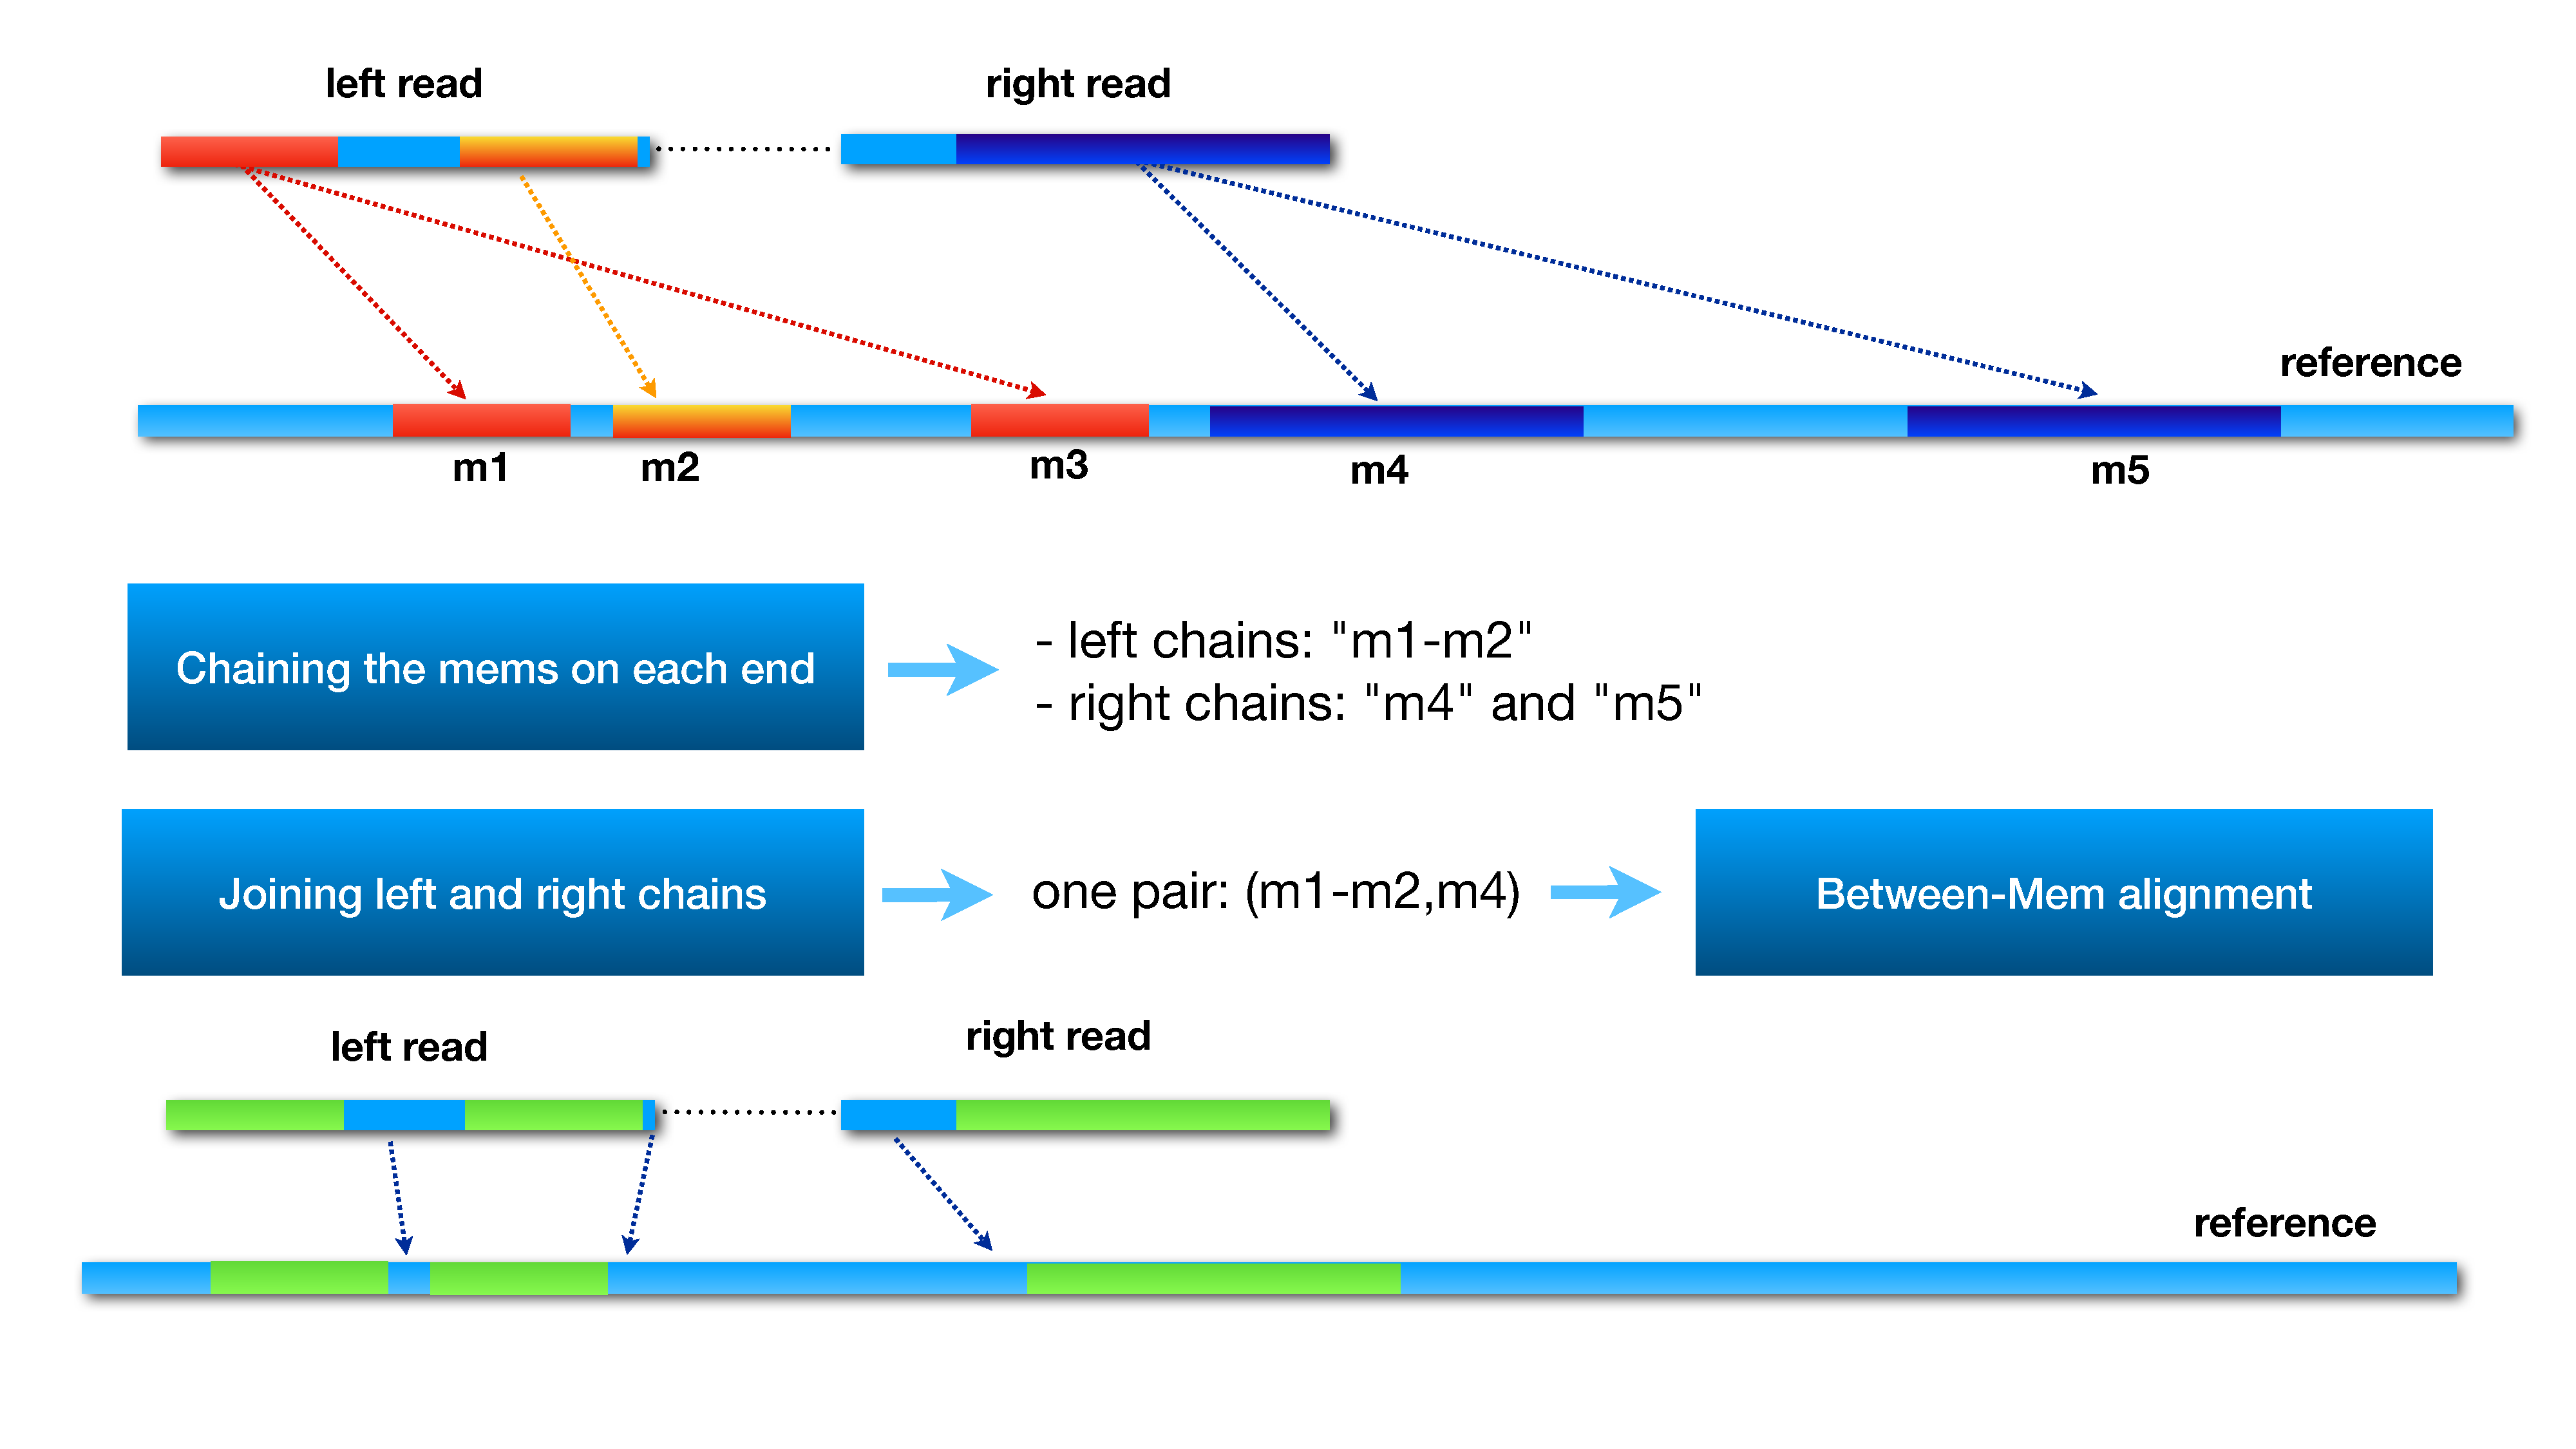
\includegraphics[width=0.95\columnwidth, trim={0in 0in 0in 0in},clip]{Figures/puff/MainFig.pdf}
    \caption[Main steps of chaining and between-\mem alignment in the \puffaligner]
    {This figure shows the main steps of chaining and
    between-\mem alignment in the \puffaligner procedure via an
    example. In this example, m1, m2 and m3 are the projected \mems
    from the left end of the read to the reference and m4 and m5 are
    the projected \mems from the right end of the read. In the first
    step, the chaining algorithm chooses the best chain of \mems that
    provide the highest coverage score for each end of the read, that
    is the m1-m2 chain for the left end and two single \mem chain for
    the right end. Then, the selected chains from each end are joined
    together to find the concordant pairs of chains, that is the
    (m1-m2, m4) pair for this read as m5 is too far from m1-m2. Then,
    the chain from each end will go through to the next step,
    between-\mem alignment. For the green areas (\mems) no alignment
    is recalculated as they are exact matches. Only the un-matched
    blue parts of the chains (those nucleotides not occurring within
    a \mem) are aligned using a modified version of \ksw. }
    \label{fig:mainScheme}
\end{figure}

In \puffaligner, if the distance between two \mems, $m_1$ and $m_2$,
on the read and the reference is $d_r$ and $d_t$ respectively, these
two \mems should not be chained together if $|d_r - d_t| > C$, where
$C$ is the maximum allowed gap. So, the penalization term, the
$\beta$ value in ~\citep{minimap2}, in the coverage score computation
is modified accordingly to prevent pairing of such \mems.

Also, unlike what is done in minimap2~\citep{minimap2}, rather than
considering together the \mems that are discovered on both ends of a
paired-end read, we consider the chaining and chain filtering for
each end of the read separately. This is done in order to make it
easier to enforce the orientation consistency of the individual
chains. Specifically, the chaining algorithm that is presented
in minimap2~\citep{minimap2} introduces a transition in the recursion that can
be used to switch between the \mems that are part of one read and
those that are part of the other. However, such switching makes it
difficult to enforce the orientation consistency of the chains that
are being built for each end of the read. One solution 
to this problem is to add another dimension to the dynamic programming
table, encoding if one has already switched from the \mems of one read end to
the other, and the recurrence can be modified to allow only one switch
from the one read end to the other, allowing enforcement of orientation
consistency. However, we found that, in practice, simply chaining the
read ends separately led to better performance.

Finally, we also adopt the heuristic proposed by minimap2~\citep{minimap2} when
calculating the highest scoring chains. That is, when a \mem is added
to the end of an existing chain, it is unlikely that a higher score
for a chain containing this \mem will be obtained by adding it to a
preceding chain. Thus, we consider only a small fixed number of
rounds (by default 2) of preceding chains once we have found the
first chain to which we can add the current \mem.

The chaining algorithm described above finds the best chains of \mems
shared between the read $r$ and the reference $t$ in orientation $o$.
A chain is accepted if its score is greater than a
configurable fraction, which we call the \textit{consensusFraction},
times the maximum coverage score found for the read $r$ to \emph{any}
reference. Throughout all the experiments in this manuscript the
\textit{consensusFraction} is set to $0.65$. If a chain passes the
consensus fraction threshold, we call it a \emph{valid} chain.
Additionally, rather than keeping all valid chains, we also filter
highly-suboptimal chains with respect to the highest scoring chain
\emph{per-reference}. All valid chains shared between $r$ and $t$ are sorted
by their scores, and chains having scores within $10\%$ 
of the highest scoring chain for reference $t$ are selected as
potential mappings of the read $r$ to the reference $t$. While these
filters are essential for improving the throughput of the algorithm
in finding the right alignment, they are carefully selected to have
very little effect on the sensitivity of \puffaligner. For
all the experiments in this manuscript, the same default settings of
these parameters are used if not mentioned otherwise.
%\mohsen{We can have an analysis of the effects of these filters in the supp}.

\subsection{Computing base-to-base alignments between \mems}
\label{subsec:base-to-base}
After finding the high-scoring \mem chains for each reference
sequence, a base-to-base alignment of the read to each of the
candidate reference sequences is computed. Each selected chain
implies a position on the reference sequence where the read might
exhibit a high quality alignment. Thus, we can attempt to compute an
optimal alignment of the read to the reference at this implied
position, potentially allowing a small bit of padding on each side of
the read. This approach utilizes the positional information provided
by the \mem chains. However, the starting position of the alignments
is not the only piece of information embedded in the chains. Rather
each chain of \mems consists of sub-sequences of the read (of size at
least $k$, though often longer) which match exactly to the reference. While the optimal
alignment of the read to the reference at the position being
considered is not \emph{guaranteed} to contain these exact matches as
alignments of the corresponding substrings, this is almost always the
case.

In \puffaligner, we aim to exploit the information from the long
matches to accelerate the computation of the alignments. In fact,
since only chains with relatively high coverage score are
selected, a large portion of the read sequences are typically already
matched to the positions in the reference with which they will be
matched in the final optimal alignment. For instance,
in~\cref{fig:mainScheme}, for the final chains selected on the
reference sequence, it is already known for the light blue, dark blue
and green sub-sequences on the left end of the read precisely where
they should align to the reference. Likewise this is the case for the yellow and
purple sub-sequences on the right read. The unmapped regions of the
reads are either bordered by the exact matches on both sides, 
or they occur at the either ends of the read sequence.
\puffaligner skips aligning the whole read sequence by considering
the exact matches of the \mems to be part of the alignment solution.
As a result, it is only required to compute the alignment of the
small unmapped regions, which reduces the computation burden of the
alignments.

When applying such an approach, two different types of alignment
problems are introduced, which we call bounded sub-sequence alignment
and ending sub-sequence alignment. For bounded sub-sequence alignment, we need
to \emph{globally} align some interval $i_r$ of the read to an
interval $i_t$ of the reference. If $i_r$ and $i_t$ are of different
lengths, the alignment solution will necessarily include insertions
or deletions. If $i_r$ and $i_t$ are of the same length, then the
optimal global alignment between them may or may not include indels.
For each such bounded sub-sequence alignment, we determine the
optimal alignment of $i_r$ to $i_t$ by computing a global pair-wise
alignment between the intervals, and stitching the resulting
alignment together with the exact matches that bound these regions.

Gaps at the beginning or the end of the read are symmetric cases, and so we
describe, without loss of generality, the case where there is an unaligned
interval of the read after the last \mem shared between the read and the
reference. In this case, we need to solve the ending sub-sequence alignment
problem. Here, the unaligned interval of the read consists of the substring
spanning from the last nucleotide of the terminal \mem in the chain, up through
the last nucleotide of the read. There is not a clearly-defined interval on
the reference sequence. While the left end of the relevant reference interval
is defined by the last reference nucleotide that is part of the bounding \mem,
the right end of the reference interval should be determined by actually solving
an extension or ``end-free'' alignment problem. We address this by performing
extension alignment of the unaligned interval of the read to an interval of the
reference that begins on the reference at the end of the terminal \mem, and
extends for the length of the unaligned query interval plus the length of some
problem-dependent buffer (which is determined by the maximum length difference  
between the read and reference intervals that would still admit an alignment
within the acceptable score threshold).

An example of both of these cases is displayed in~\Cref{fig:mainScheme}.
Specifically, an alignment of the read could be obtained by only solving two
smaller alignment problems; one is the ending sub-sequence alignment of the
unmapped region after the green \mem on the left read and the other is the
bounded sub-sequence alignment of region on the right read bordered by the
yellow and purple \mems.

\puffaligner uses \ksw~\citep{suzuki2018introducing, minimap2} for
computing the alignments of the gaps between the \mems and for aligning 
the ending sequences. \ksw exposes
a number of alignment modes such as global and extension alignments.
For aligning the bounded regions, \ksw alignment in the global mode
is performed, and for the gaps at the beginning or end of reads,
\puffaligner uses the extension mode to find the best possible
alignment of that region. \puffaligner, by default, uses a match
score of $2$ and mismatch penalty of $4$. For indels, \puffaligner
uses an affine gap scoring schema with gap open penalty of $5$ and
gap extension penalty of $3$. In \puffaligner, after computing the
alignment score for each read, only the alignments with a score
higher than $\tau$ times the maximum possible score for the read are
reported. The value of $\tau$ is controlled by the option
\textit{--minScoreFraction}, which is set to $0.65$ by default.

\subsection{Enhancing alignment computation}
\label{subsec:ksw_improvements}

By only aligning the read's sub-sequences that are not included in the \mems, the size of alignment problems being solved in \puffaligner are often much shorter than the length of the read. However, to further speed up alignment, we also incorporate a number of other techniques to improve the performance of the alignment calculation. We describe the most important of these below:

\begin{itemize}
    \item \textbf{Skipping alignment calculation by recognizing perfect chains and alignment caching:} It is possible to avoid the alignment computation completely in a considerable number of cases. In fact, as has been explained in previous work~\citep{selaln}, the alignment calculation step can be completely skipped if the set of exact matches for each chain covers the whole read. \puffaligner skips alignment for cases where the coverage score of chains of \mems is the length of the read, and assigns a total matched CIGAR string for that alignment. Alignment computation of a read might be also skipped if the same alignment problem has been already detected and computed for this read. For example, in the case of RNA seq data, reads often map to the same exons on different transcripts. In such cases, each alignment solution for a read is stored in a cache (a hash table) so that if the same alignment problem is detected, the solution can be directly retrieved from the cache, and no further computation is required (see~\cref{tab:skipped-alignments}).

    \begin{table}%[h!]
    \centering
    \begin{tabular}{lcccc}
        \toprule sample & Cache Hits & Perfect Chains & None Alignable & Total Skipped \\
        \midrule
        DNA-seq experimental & \num{52.8941105}\% & \num{19.008135}\% & \num{0.71}\% & \num{72.67}\% \\
        RNA-seq simulated & \num{28.6918391}\% & \num{50.8027558}\% & \num{0.97}\% & \num{80.46}\% \\
        Metagenomic simulated & \num{61.095958}\% & \num{31.3338897}\% & \num{0.0} \% & \num{92.43}\% \\
        \bottomrule
    \end{tabular}
    \caption[he percentage of skipped aligner engine calls]{The percentage of aligner engine calls skipped in the alignment calculation pipeline.}
    \label{tab:skipped-alignments}
    \end{table}

    %As noted in table (tab:skipped-alignments) up to 75 percent of alignment companions is skipped by considering the perfect chains and the alignment cache.
    \item \textbf{Early stopping of the alignment computation when a valid score cannot be achieved:} While care is taken to produce only high-scoring chains between the read and reference, it is nonetheless the case that the majority of the chains do not lead to an alignment of acceptable quality. Since the minimum acceptable alignment score is immediately known based on $\tau$ and the length of the read, the base-to-base alignment calculation can be terminated at any point where it becomes imposible for the minimum required alignment score to be obtained. This approach can be applied both during the \ksw alignment calculation, and also after the alignment calculation of each gap is completed. During this procedure, for each base at position $i$, starting from position $1$ on the read of length $n$, if the best alignment score $p$ up to the $i$-th position is $s_i$, we can calculate the maximum possible alignment score, $s_{max}$, that might be achieved starting at this location given the current alignment score by:
    \begin{equation}
        s_{max} = s_i + MS * (n - s_i),
    \end{equation}
    where $MS$ is the score assigned to each match. If $s_{max}$ is smaller than minimum required score for accepting the alignment, the alignment calculation can be immediately terminated, since it is already known that this anchor is not going to yield a valid alignment for this read.

    \item \textbf{Full-sensitivity banded alignment:} \ksw is able to perform banded 
    alignment to make alignment calculation more efficient. In this mode, the dynamic 
    programming matrix for the alignment problem is only filled out along the sub-diagonals 
    out to a certain distance $d$ away from the main diagonal. If one is guaranteed that any 
    valid alignment must have fewer than $d$ insertions or deletions, then the alignment must 
    not exit these bands of the dynamic programming matrix.  Note that alignments with 
    $> d$ indels can be represented within these bands as insertions and deletions move 
    in opposite anti-diagonal directions, but it is certainly the case that no alignment
    with $\le d$ indels can exit these bands. By calculating the maximum number of gaps 
    (insertions or deletions) allowed in each sub-alignment probem, in a way that we are 
    certain that any alignment having greater than this number of gaps must drop below 
    the acceptable threshold, we utilize the banded alignment in \ksw within each 
    sub-alignment problem without losing any sensitivity with respect to non-banded alignment.
\end{itemize}

\subsection{Joining mappings for read ends and orphan recovery}
\label{subsec:orphan_recovery}
Finally, once alignments have been computed for the individual ends
of a read, they must be paired together to produce valid alignments
for the entire fragment. At this point in the process, on each
reference sequence, there are a number of locations where the left
end of each read or the right end of each read, or both, are mapped 
to the reference. For the
purpose of determining which mappings will be reported as a valid
pair, the mappings are joined together only if they occur on opposite
strands of the reference, and if they are within a maximum allowed
fragment length. There are two different types of paired-end
alignments that can be reported by \puffaligner; concordant and
discordant. If \puffaligner is disallowed from reporting discordant
alignments, then the mapping orientation of the left and right end
should agree with the library preparation protocols of the reads.
\puffaligner first tries to find concordant mapping pairs on a
reference sequence, and if no concordant mapping is discovered and
the tool is being run in a mode where discordant mappings are
allowed, then \puffaligner reports pairs that map discordantly. Here,
discordant pairs may be pairs that do not, for example, obey the
requirement of originating from opposite strands. While this is not
expected to happen frequently, it may occur if there has been an
inversion in the sequenced genome with respect to the reference.

\paragraph{Orphan recovery: }  If there is no valid paired-end alignment for a fragment 
(either concordant or discordant, if the latter is allowed), then \puffaligner will attempt to 
perform orphan recovery. The term ``orphan'' refers to one end of paired-end read that is confidently 
aligned to some genomic position, but for which the other read end is not aligned nearby (and paired). 
To perform orphan recovery, \puffaligner examines the reference sequence downstream of the mapped read 
(or upstream if the mapped read is aligned to the reverse complement strand) and directly performs dynamic 
programming to look for a valid mapping of the unmapped read end. For this purpose, we use the ``fitting'' 
alignment functionality of edlib~\citep{edlib} to perform a simple Levenshtein distance based alignment that 
will subsequently be re-scored by \ksw. Finally, if, after attempting orphan recovery, there is still no valid 
paired-end mapping for the fragment, then orphan alignments are reported by \puffaligner (unless the 
``\conf{--noOrphans}'' flag is passed).

\subsection{Assessing \puffaligner's performance}

For measuring the performance of \puffaligner and comparing it to other aligners, we have designed a 
series of experiments using both simulated and experimental data from different sequencing assays. We compare 
\puffaligner with \bt~\citep{bowtie2}, \st~\citep{star} and \debga~\citep{debga}. \bt is a popular, sensitive 
and accurate aligner with the benefit of having very modest memory requirements. \st requires a much larger 
amount of memory, but is much faster than \bt and can also perform ``spliced alignment" against a reference 
(which \puffaligner, \bt, and \debga currently do not allow). \debga, is most-related tool to \puffaligner 
conceptually, as it is an aligner with a \ccdbg-based index that is focused on exploiting redundancy in the 
reference sequence.

We use different metrics to assess both the performance and accuracy of each method on a variety of types of 
sequencing samples. These experiments are designed to cover a variety of different use-cases for an aligner, 
spanning the gamut from situations where most alignments are expected to be unique (DNA-seq), to situations 
where each fragment is expected to align to many loci with similar quality (RNA-seq and metagenomic sequencing), 
and spanning the range of index sizes from small transcriptomes to large collections of genomes.

First, we show \puffaligner exhibits similar accuracy for aligning DNA-seq reads to \bt, but it is considerably 
faster. In the case of experimental reads, since the true origin of the read is unknown, we use measures such as 
mapping rate and concordance of alignments to compare the methods. Furthermore, we evaluate the accuracy of 
aligners by aligning simulated DNA-seq reads that include variation (single-nucleotide variants and small indels 
with respect to the reference). For aligning RNA-seq reads, we compare the impact of alignments produced by each 
aligner on downstream analysis such as abundance estimatation. Finally, we show \puffaligner is very efficient for 
aligning metagenomic samples where there is a high degree of shared sequence among the reference genomes being 
indexed. We also illustrate that using alignments produced by \puffaligner yields the highest accuracy for 
abundance estimation of metagenomic samples.

\subsection{Configurations of aligners in the experiments}

The performance of each tool is impacted by the different alignment scoring schemes they use, e.g. 
different penalties for mismatches, and indels. To enable a fair comparison, we attempted to configure 
the tools so as to minimize divergences that simply result from differences in the scoring schemes. For 
the experiments in this section, we use \bt in a near-default configuration (though ignoring quality values), 
and attempt to configure the other tools, as best as possible, to operate in a similar manner.

The \debga scoring scheme is not configurable, so we use this aligner in the default mode (unfortunately, 
the inability to disable local alignment and forcing just computation of end-to-end alignments in \debga makes 
certain comparisons particularly difficult). For \puffaligner we use a scheme as close to \bt as possible. The 
maximum possible score for a valid alignment in \bt is $0$ (in end-to-end mode) and each mismatch or gap subtracts 
from this score. \bt uses an affine gap penalty scoring scheme, where opening and extending a gap (insertion or 
deletion) have a cost of $5$ and $3$ respectively. For DNA-seq reads, we configure \st to allow as many mismatches 
as \bt and \puffaligner by setting the options ``\conf{--outFilterMismatchNoverReadLmax 0.12}'' and 
``\conf{--outFilterMismatchNmax 1000}''. Also, we use ``\conf{--alignIntronMax 1}'' in \st to perform 
non-spliced alignments while aligning genomic reads. For RNA-seq reads, \st has a set of parameters which 
we change in our result evaluations, and which are detailed below in the relevant sections.

In \bt we also use the option \conf{--gbar 1} to allow gaps anywhere on the read except within the first 
nucleotide (as the other tools have no constraints on where indels may occur). Furthermore, for consistency, 
we also run \bt with the option ``\conf{--ignore-quals}'', since the other tools do not utilize base qualities 
when computing alignment scores.

As explained in~\Cref{par:repetitivehits}, for the sake of performance, highly repeated anchors 
(more than a user-defined limit) will be discarded before the alignment phase.
This threshold is by default equal to $1000$ in \puffaligner. We set the threshold to the same 
value for \st and \debga using options \conf{--outFilterMultimapNmax 1000} and \conf{-n 1000} 
respectively. There is no such option exposed directly in \bt.

Since \puffaligner finds end-to-end alignments for the reads, we are also running other tools in end-to-end 
mode, which is the default alignment mode in \bt as well. In \st we enable this mode using the option 
\conf{--alignEndsType EndToEnd}. In the case of \debga, although the documentation suggests it is \emph{not} 
supposed to find local alignments by default, the output SAM file contains many reads with relatively long 
soft clipped ends, so if a read is not aligned end-to-end, \debga reports the local alignment for that.
We were not able to find any option to force \debga to perform end-to-end alignments for all reads, and 
so we have compared it in the configuration in which we were able to run it.

For aligning DNA-seq samples, each aligner is configured to report a single alignment, which is the primary 
alignment, for each read. \bt outputs one alignment per read by default. To replicate this in the other tools, 
we use the option \conf{--outSAMmultNmax 1} in \st, \conf{-o 1 -x 1} in \debga, and \conf{--primaryAlignment} 
in \puffaligner.

\subsection{Alignment of whole genome sequencing reads}

First, we evaluate the performance of \puffaligner with a whole genome sequencing (WGS) sample from 
the $1000$ Genomes project~\citep{10002015global}. We downloaded the \texttt{ERR013103} reads from sample 
\texttt{HG00190}, which is a low-coverage sample from a Finnish male, sequenced in Finland.
\footnote{https://www.internationalgenome.org/data-portal/sample/HG00190}. 
There are $18,297,585$ paired-end reads, each of length $108$ nucleotides in this sample. 
Using fastp~\citep{chen2018fastp}, we remove low quality ends and adapter sequences from these reads. 
After trimming, there are $15,404,412$ reads remaining in the sample. Indices for each of the tools 
are built over all DNA chromosomes of the latest release of the human genome (v33) by 
gencode\footnote{https://www.gencodegenes.org/human/release\_33.html}~\citep{frankish2019gencode}.

In this experiment, all aligners are configured report only concordant alignments, i.e., only pairs of 
alignments that are cocordant and within the ``maximum fragment length'' shall be reported. The maximum 
fragment length in all aligners is set to $1000$, using the option \conf{--alignMatesGapMax 1000} in \st, 
\conf{--maxins 1000} in \bt and \conf{-u 1000 -f 0} in \debga. The default value for the maximum fragment 
length in \puffaligner is set to 1000, the user can cofigure this value by using the flag 
\conf{--maxFragmentLength}. This concordance requirements also prevents \bt, \puffaligner, and \st from 
aligning both ends of a paired end read to the same strand.

The alignment rate, run-time memory usage and running time for all the aligners are presented 
in~\cref{Tab:dnaseq-exp}. The reason that \debga has the highest mapping rate in~\cref{Tab:dnaseq-exp} 
compared to other tools is that it is local alignments for the reads that are not alignable end-to-end 
under the scoring parameters for the other tools.
\bt and \puffaligner are both able to find end-to-end alignments for about $\sim95\%$ of the reads.
\st and \puffaligner are the fastest tools, with \st being somewhat faster than \puffaligner.
On the other hand, \puffaligner is able to align more reads than \st, while requiring less than half as 
much memory. The memory usage of \bt is the smallest, since \bt's index does not contain a hash table. 
However, this comes at the cost of having the longest running time compared to other methods.
Overall, \puffaligner benefits from the fast query of hash based indices while its run-time memory usage, 
which is mostly dominated by the size of the index, is significantly smaller than other hash based aligners.
Although \debga's index is based on the \dbgs, similar to the \pufferfish index, the particular encoding for 
it is not as space-efficient as that of \pufferfish.

\begin{table}%[h!]
    \centering
    \begin{tabular}{lccc}
        \toprule aligner & mapping-rate$(\%)$ & time (mm:ss) & memory (GB) \\
        \midrule
        %\puffaligner & \num{95.5495997} & 5:46 & \num{18.297428131}\\
        \puffaligner & \num{95.5831096} & 6:14 & \num{13.090557098}\\
        \debga & \num{99.7533823} & 10:46 & \num{41.040790558}\\
        \st& \num{93.880883} & 4:29 & \num{30.358268738}\\
        \bt& \num{95.4425394} & 16:15 & \num{3.5005874634}\\
        \bottomrule
    \end{tabular}
    \caption[The performance of different aligners with experimental DNA-seq reads]{The performance of different tools for aligning experimental DNA-seq reads. The time reports are benchmarked after warming up the system cache so that the influence of index loading time is mitigated.}
        \label{Tab:dnaseq-exp}
\end{table}

\begin{figure}
    \centering
    \scalebox{0.5}{
%    \includegraphics[width=0.4\linewidth,, trim={0in 0in 0in 0in},clip]
    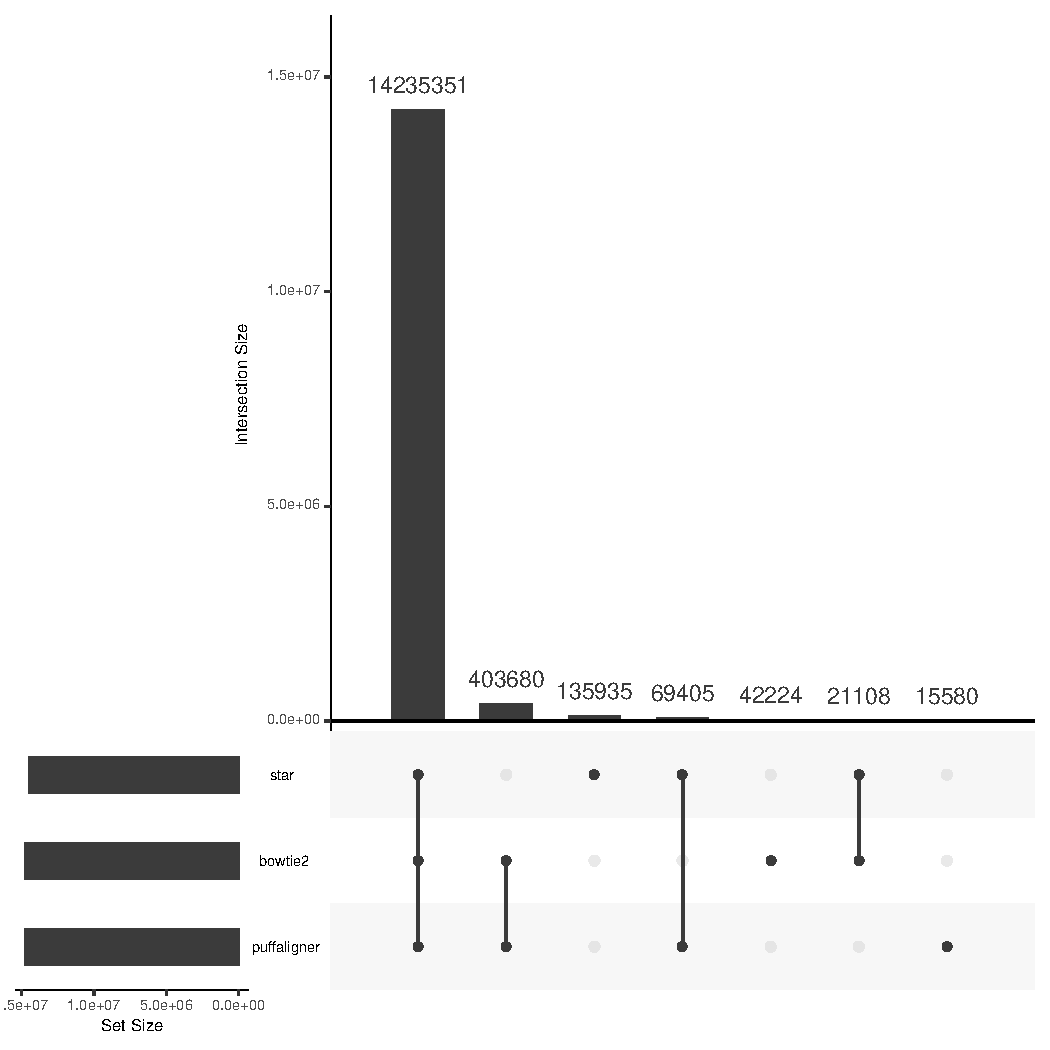
\includegraphics[trim={0in 0in 0in 0in},clip]
    {Figures/puff/ERR013103_trimmed_gencode_3tools_sparse_resubmission.pdf}}
    \caption[Upset plots for comparing the alignments - reads agreement]
    {Caomparing the alignments in terms of 
    agreement of the alignments found by different tools for each read.}
    \label{fig:upset1}
\end{figure}
\begin{figure}
    \centering
    \scalebox{0.5}{
%    \includegraphics[width=0.4\linewidth, trim={0in 0in 0in 0in},clip]
    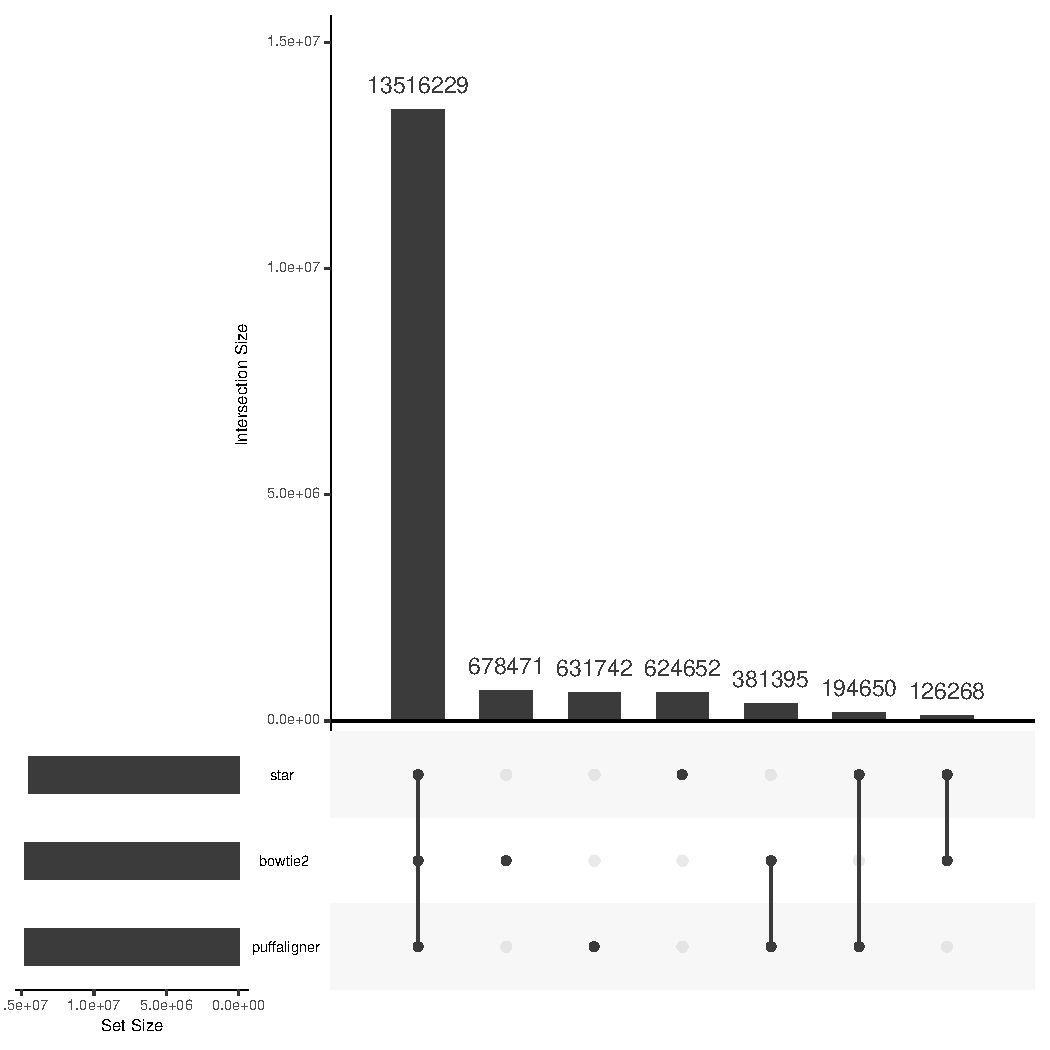
\includegraphics[trim={0in 0in 0in 0in},clip]
    {Figures/puff/ERR013103_trimmed_gencode_3tools_sparse_resubmission_location.pdf}}
    \caption[Upset plots for comparing the alignments - location agreement]
    {Caomparing the alignments in terms of 
    agreement of the alignments found by different tools based on the location of the mappings.}
    \label{fig:upset1-location}
    \label{upsetplots}
\end{figure}

To look more closely how the mappings between the tools differ, we investigate the agreement of the reads 
which are mapped by each tool and visualize the results in an upset plot in~\cref{fig:upset1} using the 
UpsetR library~\citep{conway2017upsetr}.  We are only comparing the three methods which perform end-to-end 
alignment in this plot, since outliers from the local alignments computed by \debga would otherwise dominate 
the plot. The first bar shows that the majority of the reads are mapped by all three tools.
The next largest set represents the reads which are only mapped by \bt and \puffaligner. All the other sets 
are much smaller compared to the first two sets. This fact illustrates that the highest agreement in the 
aligners is between \bt and \puffaligner. Exploring a series of individual reads from the smaller sets in 
the upset plot, suggests that some of these differences happen as a result of small differences in the scoring 
configuration, while some result from different search hueristics adopted by the different tools.
~\cref{fig:upset1-location} shows the coherence between the alignments reported by the tools by also including 
the exact location to which the reads are aligned in the reference.



\subsection{Alignment of simulated DNA-seq reads in the presence of variation}

To further investigate the accuracy of the aligners, we used simulated DNA-seq reads. One of the main 
differences between simulated reads and experimental reads is that simulated reads are often generated 
from the same reference sequences to which they are aligned, with the only differences being due to 
(simulated) sequencing error.  While (simulated) sequencing error prevents most reads from being exact 
substrings of the reference, it actually does not tend to complicate alignment too much.
On the other hand, while dealing with experimental data, the genome of the individual from which
the sample is sequenced might include different types of variations with respect to the reference 
genome to which we are aligning~\citep{srivastava2019alignment}. Therefore, it is desirable to introduce 
variations in the simulated samples, and to measure the robustness and performance of the different 
aligners in the presence of the variation. \mason~\citep{holtgrewe2010mason} is able to introduce different 
kinds of variations to the reference genome, such as SNVs, small gaps, and also structural variants (SV) 
such as large indels, inversions, translocations and duplications. We use \mason to simulate $9$ DNA-seq 
samples with different variation rates ranging from $1e-7$ to $1e-3$. Each sample includes $1M$ paired-end 
Illumina reads of $100$bp length from chromosome 21 of the human genome, ensembl release 98
\footnote{ftp://ftp.ensembl.org/pub/release-98/fasta/homo\_sapiens/dna/}. 

\begin{figure}%[H]
    \scalebox{0.8}{
    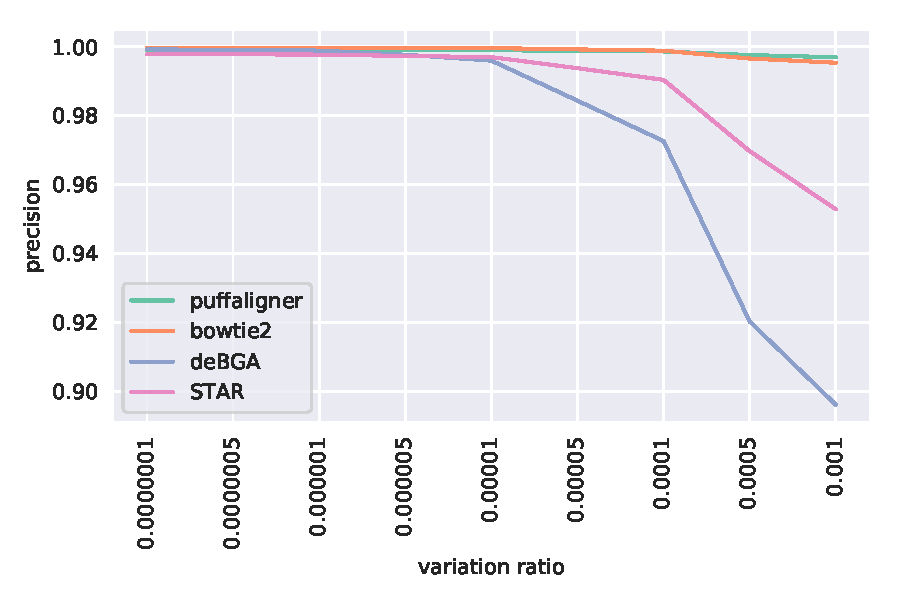
\includegraphics[width=\textwidth,type=pdf,ext=.pdf,read=.pdf]{Figures/puff/DNAseq-sim-chr21-SV-prec}}
    \caption[Accuracy of aligners in the presence of variations in the reference - precision]
    {Comparing the accuracy of aligners in the presence of different rates of variations in the reference genome
    in terms of the precision of the alignments reported by each aligner. 
    True positives (TP) are the compatible reads that are aligned to the original location, 
    and the FP set consists of both the compatible reads aligned to sub-optimal locations 
    (alignments with larger edit distance than the alignment to the original location) 
    and the non-compatible reads that are aligned with high ($>25$) edit distance.}
\end{figure}
\begin{figure}%[H]
    \scalebox{0.8}{
    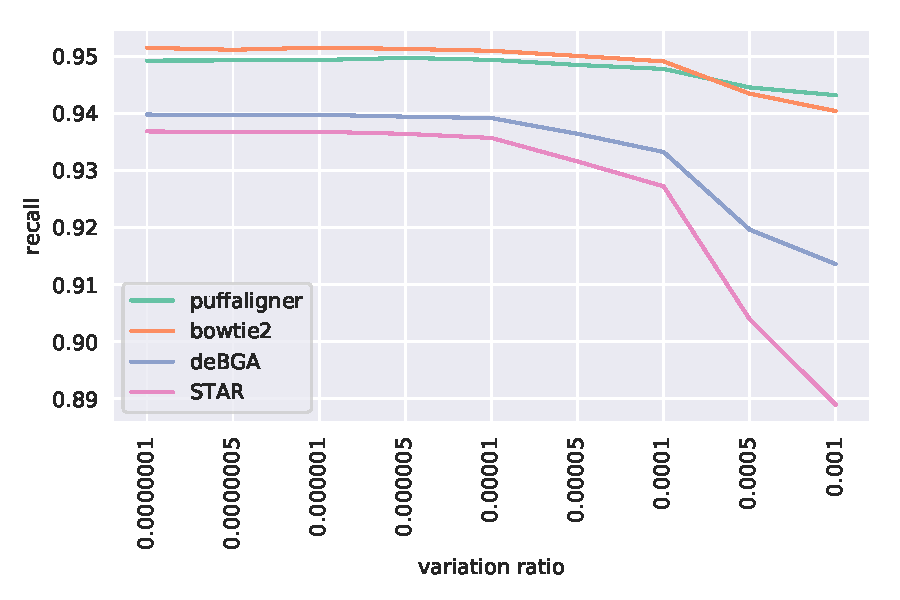
\includegraphics[width=\textwidth,type=pdf,ext=.pdf,read=.pdf]{Figures/puff/DNAseq-sim-chr21-SV-recall}}
    \caption[Accuracy of aligners in the presence of variations in the reference - recall]
    {Comparing the accuracy of aligners in the presence of different rates of variations in the reference genome
    in terms of the ratio of the alignments in the true SAM file that are recovered by each aligner. 
    The recall is the result of dividing the number of TP reads by the total number of compatible reads.}
    \label{fig:DNAseq-SV}
\end{figure}

For this analysis, we do not restrict the aligners to only report concordant alignments, since the structural variations in the samples can lead to valid discordant alignments, such as those on
the same strand or with inter-mate distances larger than the maximum fragment length. To be specific, we do not use the options which limit \bt and \puffaligner to report only concordant alignments, in addition, we use the option ``\conf{--dovetail}'' in \bt to consider dovetail pairs as concordant pairs. 

The alignments reported by \debga already include discordant pairs and also orphan mappings. Furthermore, To remove any restrictions on the fragment length in the alignments reported by \debga, we set the minimum and maximum insert size, respectively to 0 and the 50000, since setting a larger value resulted in the tool running into segmentation fault. 

To allow dovetail pairs and also larger gaps between the pairs in \st, we use the following options:\\
``\conf{--alignEndsProtrude 1000000 ConcordantPair}''\\
``\conf{--alignMatesGapMax 1000000}''\\
By default there is not a specific option in \st for allowing orphan alignment of paired end reads. Instead, we can increase the number of allowed mismatches to be as large as one end of the read by using the following options:\\
``\conf{--outFilterMismatchNoverReadLmax 0.5}''\\
``\conf{--outFilterMismatchNoverLmax 0.99}''\\
``\conf{--outFilterScoreMinOverLread 0}''\\
``\conf{--outFilterMatchNminOverLread 0}''

For each sample, \mason produces a SAM file which includes the alignment of the simulated reads to the original, non-variant version of the reference --- the version which was used for building the aligner’s indices in this experiment. Based on the alignments reported in the truth file, some reads did not have a valid alignment to the original reference. This was the result of a high rate of variations at some sequencing sites. We called the set of reads that, according to the truth SAM file, were aligned to the original reference as compatible reads.

We compared the performance of aligners based upon how well they are able to align the compatible reads. We computed the precision and recall of the alignments reported for these reads as follows. True positives are considered the reads that are mapped by the aligner to the same location stated by the truth file. Then, recall is computed by dividing the number of true positives by the number of all compatible reads. Furthermore, we considered an alignment as a false positive in two different cases. First, an alignment was considered discordant if the reported alignment had a large edit distance (larger than 25) for the non-compatible reads. Second, in the case that an aligner reported an alignment to a location other than the one in the truth file, it was considered as a false positive if the edit distance of the reported alignment is greater than the edit distance of the true alignment. Having defined the set of TP and FP for the alignments, and also having considered the set of all compatible reads as the set we are trying to recover, we computed precision and recall for the set of alignments reported by each aligner.

~\Cref{fig:DNAseq-SV} shows the precision and recall of the aligners for different samples. 
According to~\cref{fig:DNAseq-SV}, for lower variation ratios up until $10e-5$, most of the tools are 
able to make accurate alignment calls with a high specificity. As the variation ratio introduced in the 
sample is increased, all the tools start to have lower precision and recall.
\debga and \st perform worse in higher variation samples, as they fail to recover the true alignment for more 
reads, while \bt and \puffaligner are able to align most of the reads to their true 
location on the original reference.

These results show that \puffaligner' accuracy is stable in the face of variation which makes the tool 
suitable for datasets that are known to have substantial variation, such as when aligning reads to 
microbial genomes where the specific sequenced strain may not be represented in the reference set.

\subsection{Quantification of transcript abundance from RNA-seq reads}

Mapping sequencing reads to target transcriptomes is the initial step in many pipelines for reference-based 
transcript abundance estimation. While lightweight mapping approaches~\citep{kallisto,salmon} greatly speed-up 
abundance estimation by, in part, eliding the computation of full alignment between reads and transcripts, 
there is evidence that alignments still yield the most accurate abundance estimates by providing increased 
sensitivity and avoiding spurious mappings~\citep{selaln,revisit,srivastava2019alignment}. Thus, the continued 
development of efficient methods for producing accurate transcriptome alignments of RNA-seq reads remains a 
topic of interest. In this section, we compare the effect of alignments produced by each tool on the accuracy 
of RNA-seq abundance estimation.  

We generated \num{9968245} paired-end RNA-seq reads using the polyester~\citep{polyester} read simulator. 
The reads are generated by the \conf{simulate experiment countmat} module in polyester.
The input count matrix is calculated based on the estimates from the \bt-\salmon pipeline on the sample 
\texttt{SRR1085674} (where reads are first aligned with \bt and then the alignments are quantified using 
\salmon). This sample is a collection of paired-end RNA-seq reads sequenced from human transcriptome using 
an Illumina HiSeq~\citep{lonsdale2013genotype}.
The human transcriptome from gencode release (33) is used to build all the aligners' indices. Also, for 
building \st's index in the genome mode, the human genome and the comprehensive gene annotation 
(main annotation file) is obtained from the same release of gencode.

\begin{table}
    \centering
    \begin{tabular}{lcccc}
        \toprule aligner & spearman & MARD & time (mm:ss) & memory (GB) \\
        \midrule
        \puffaligner & \num{0.920247842672} &  \num{0.0524302645945} & 1:17 & \num{2.5428848267}\\
        \debga & N/A & N/A & 5:19 & \num{9.9649429321}\\
        \st - transcriptome & \num{0.920269439222} & \num{0.052751264979} & 1:57 & \num{8.7343559265}\\
        \st - genome & \num{0.900578269027} & \num{0.0641767676706} & 3:30 & \num{32.573215485}\\
        \bt& \num{0.919895559666} & \num{0.0526921568832} & 32:59 & \num{1.1455192566}\\
        \bottomrule
    \end{tabular}
    \caption[Abundance estimation of simulated RNA-seq reads]{Abundance estimation of simulated RNA-seq reads, computed by \salmon, using different tools' alignment outputs. The time and memory are only for the alignment step of each tool and the time for abundance estimation by \salmon is not considered.}
    \label{Tab:rnaseq-quant}
\end{table}

As the reads in this experiment are RNA-seq reads sequenced from the human transcriptome, it is important 
to account for multi-mapping, as often, a read might map to multiple transcripts which share the same exon 
or exon junction.
This property makes the direct evaluation of performance at the level of alignments difficult.
Therefore, a typical approach in evaluating the accuracy of the transcriptomic alignments is to assess the 
accuracy of downstream analysis such as abundance estimations by computing the correlation and relative 
differences of the estimates with the true abundance of the transcripts.
To compare the accuracy of each tool we give the alignments produced by each aligner, which are in the SAM 
format, as input to \salmon to estimate the transcript expressions.

\puffaligner, by default, outputs up to 200 alignments with an alignment score greater than $0.65$ times the 
best alignment score, i.e., the alignment for the read in the case that all bases are perfectly matched to the 
reference.
To enable the multi-mapping to take into account the characteristics of alignment to the transcriptome,
\bt is run with the option \conf{-k 200} which lets the tool output up to $200$ alignments per read. The 
value of $200$ is adopted from the suggested parameters for running RSEM~\citep{rsem} with \bt alignments. 
We note that running \bt with this option makes the tool considerably slower than the default mode, as many 
more alignments will be computed and output to the SAM file under this configuration.
For both \bt and \puffaligner, and also for \st by default, orphan and discordant mappings are not allowed.

We ran \st with the \conf{`ENCODE`} options, which are recommended in the \st manual for RNA-seq reads.
\st is also run in two different modes, one is by building the \st index on human genome, while it is also 
provided a GTF file for gene annotation. In this mode, \st performs spliced alignment to the genome, then 
projects the alignments onto transcriptomic coordinates. The other mode is building the \st index on the 
human transcriptome directly, which allows \st to align the RNA-seq reads directly to the transcripts in an 
unspliced manner. We chose to run \st in the transcriptomic mode as well, since we find that it yields higher 
accuracy, though this increases the running time of \st.

The \debga index is built on the transcriptome, as are the \bt and \puffaligner indices, since these tools 
do not support spliced read alignment. \debga is run in the with options \conf{-o 200 -x 200}, which nominally 
has the same effect as \conf{-k 200} in \bt, according to the documentation of \debga.

Accuracy of abundance estimation by \salmon, when provided the SAM output generated by each aligner, is 
displayed in~\cref{Tab:rnaseq-quant}. The timing and memory benchmarks provided in this table is only for the 
alignment step. Alignments produced by \puffaligner, \bt and \st in the transcriptomic mode produce the best 
abundance estimates. \debga's output alignments are not suitable for any abundance estimation as many reads 
are aligned only to the same strand which are later filtered during the abundance estimation by \salmon, so 
we could not provide a meaningful correlations for abundance estimation using \debga's alignments.
Aligning the reads by \st to genome and then projecting to transcriptomic coordinates does not generate as 
high correlation as directly aligning the reads to the transcriptome by \st.  However, we note that, as 
described by~\citet{srivastava2019alignment}, there are numerous reasons to consider alignment to the 
entire genome that are not necessarily reflected in simulated experiments.
While the memory usage by \puffaligner is only 2 fold larger than memory used by \bt, it computes the 
alignments much more quickly. 

According to the results in~\cref{Tab:rnaseq-quant} \puffaligner is the fastest aligner in these benchmarks, 
and the accuracy as high as \bt and \st for aligning RNA-seq reads.  Here, \puffaligner leads to the most 
accurate abundance estimates, while being $30$ times faster than \bt. Moreover, The memory usage is much 
less than other fast aligners such as \st.

\subsection{Alignment to a collection of microorganisms --- simulated short reads}

To demonstrate the performance and accuracy of \puffaligner for metagenomic samples, we designed two different 
experiments. One main property of metagenomic samples is the high similarity of the reference sequences against 
which one typically aligns, where a pair (or more) of references may be more than $90\%$ identical.
The first experiment we designed for this scenario, to specifically evaluate issues related to this challenge, 
we call the ``single strain'' experiment. Additionally, metagenomic samples also have the property of containing 
reads from a variety of genomes, some of which are not even assembled yet -- and hence unknown. This leads to 
the second experiment, which we call the ``bulk'' experiment, that compares the aligners in the presence of a 
high variety of \texttt{species} in the sample in addition to the high similarity of references.

For simplicity and uniformity, all the experiments have been run in the concordant mode for both \puffaligner 
and \bt (both of which support such an option), disallowing orphans and discordant alignments.
All aligners are run in three different confiurations, allowing three specific maximum numbers of alignments per 
fragment; 1 (primary output with highest score, breaking ties randomly), 20, and 200.
\puffaligner and \st, as the only tools that support this option, also are run in the \emph{bestStrata} mode.
In this mode, the aligner outputs all \emph{equally-best} alignments for a read with highest score without the 
limitation on number of reported alignments. This option is inspired by the similarly-named option in 
Bowtie1~\citep{langmead2010aligning}. However, unlike Bowtie1, \puffaligner and \st only make a best-effort 
attempt to find the score of the best stratum alignments, and do not guarantee to find the best stratum 
(though the cases in which they fail to seem to be exceedingly rare). This option is especially useful in 
the metagenomic analyses, as we will report only the best-score alignments without having an arbitrary 
limitation on the number of allowed alignments. This allows proper handling of highly multi-mapping 
metagenomic reads. In other words, using this option, one can achieve a high sensitivity without the need to 
hurt specificity. The details of each experiment is explained in the following sections.

\subsection{A single-strain Experiment}

For this experiment, we download the viral database from NCBI,
and choose three similar coronavirus genomes.
This set includes one of the recently-uploaded samples from Wuhan~\citep{wu2020new,baranov2005programmed}.
We select three very similar viral genomes to simulate reads from, which are: NC\_045512.2, NC\_004718.3, 
and NC\_014470.1. There are also a lot of literature discussing the similarity in sequence and behavior for 
these three species of coronavirus~\citep{wang2020unique,zhang2020probable,tang2020origin}.
The first is the complete genome for severe acute respiratory syndrome coronavirus 2 isolate Wuhan-Hu-1
known as Covid19 with length of $29,904$ bases. NC\_004718.3 is the ID of SARS coronavirus complete genome 
(length: $29,752$) and finally, NC\_014470.1 is a Bat coronavirus BM48-31/BGR/2008 complete genome 
(length: $29,277$).

We use \mason~\citep{holtgrewe2010mason} to generate three simulated samples,
each sample contains $500,000$ reads only from one of the three viral references 
we mentioned earlier. Then, reads were aligned back to the database of viral 
sequences using each of the four aligners. The results are shown in~\cref{tab:single-alignment-accuracy} 
for the reads simulated from the covid19 strain.

As the results show, the alignments of all aligners, except for \debga, are distributed only 
across the three references of interest out of all the reference sequences in the complete viral database.
\debga reports only a few alignments to a forth virus.  In general, all of the aligners do 
a good job of reporting the correct alignment among the returned alignments for each read.
Here, we are more interested in exploring how sub-optimal alignments are computed and 
filtered under different settings when aligning to a collection of very similar genomes.
The results show that all tools have very high sensitivity even when considering only 
a single (primary) alignment per read.  As we allow more alignments to be reported, 
the sensitivity increases and quickly levels off for all the tools.  On the other hand, 
more alignments are generated and \bt, in particular, generates a considerable number 
of extra alignments as the maximum number of allowed reported alignments is increased.
However, the results do not change when allowing more than 20 alignments, 
which means no more than 20 alignments ever pass the alignment score threshold for these reads in the 
viral database for any of the tools we are testing. 
    
The results indicate that, when allowing more than one alignment to be reported for every read, \bt
tends to report a large number of sub-optimal (yet, still valid) alignments compared to other tools. 
These are alignments that are accepted within the alignment score threshold, but are to another target 
than the one from which the read truly originates. Generating these sub-optimal alignments is in no way 
wrong, but it has a non-trivial computational cost, as shown in~\cref{fig:alignment_performance}, even if 
these alignments are not used in downstream analysis. Further, the score of the best alignment for each 
read is specific to that read and not known ahead of time, meaning that this situation cannot be completely 
addressed simply by setting more stringent parameters for which alignment scores should be allowed. 
This behavior of \bt gives the other tools a computational advantage when the user only truly requires 
the set of equally-best alignments for each read.
    
Interestingly, there is one read that all tools, except for \puffaligner fail to properly align.
Inspecting this alignment reveals it is a valid alignment within the range of the acceptable scoring 
threshold, and it is unclear why it is not discovered by the other tools. Overall, the aligners tested 
perform very well here in reporting the true strain of origin without reporting too many extra alignments. 
Interestingly, despite changing the parameters to allow more alignments, \st tends to return the same set 
of alignments under all configurations in this experiment.~\Cref{fig:alignment_performance} shows 
that \puffaligner has the lowest running time, even when the number of allowed alignments per read increases.

\paragraph{BestStrata Mode}

In this small example, all tools showed good sensitivity (and 
\puffaligner and \st showed near-perfect sensitivity) even when reporting
only a single-alignment per read. This experiment is, of course, an
atypically small test for multi-mapping read. In in larger samples, with
reads deriving from more organisms and a larger database of references,
permitting more alignments usually yields non-trivial improvements in
sensitivity. To control the rate of reporting sub-optimal alignments,
\puffaligner supports the ``best strata'' option -- also available to
\st, which allows only the alignments with the best calculated score to
be reported (as a replacement for maximum allowed number of alignments).
Using this option, \puffaligner achieves full specificity and sensitivity
in this experiment~\cref{tab:single-alignment-accuracy}.
We further demonstrate the positive impact of this option on the
alignment of bulk metagenomic samples in the next section.

\begin{table}%[h!]
    \centering
    \begin{tabular}{l|l|cccc}
        \toprule
        Alignment Mode 
        &
        Tool
        &
        NC\_045512.2
        &
        NC\_004718.3
        &
        NC\_014470.1
        &
        Others
        \\
        \midrule
        \multirow{4}{*}{Primary} &
        \puffaligner & \num{500000} & \num{0} & \num{0} & \num{0} \\
        &\bt & \num{499981} & 18 & \num{0} & \num{0} \\
        &\st & \num{499999} & 0 & \num{0} & \num{0} \\
        &\debga & \num{499991} & 0 & 0 & 9 \\
        \cline{1-6}
        \multirow{4}{*}{Up to 20} &
        \puffaligner & \num{500000} & \num{134} & \num{46} & \num{0}  \\
        &\bt & \num{499999} & \num{21461} & \num{2311} & \num{0}  \\
        &\st & \num{499999} & \num{0} & \num{0} & \num{0} \\
        &\debga & \num{499991} & \num{0} & \num{0} & \num{9}  \\
        \cline{1-6}
        \multirow{4}{*}{Up to 200} &
        \puffaligner & \num{500000} & \num{134} & \num{46} & \num{0}  \\
        &\bt & \num{499999} & \num{21461} & \num{2311} & \num{0}  \\
        &\st & \num{499999} & \num{0} & \num{0} & \num{0} \\
        &\debga & \num{499991} & \num{0} & \num{0} & \num{9}  \\
        \bottomrule
        \multirow{2}{*}{Best strata} &
        \puffaligner & \num{500000} & \num{0} & \num{0} & \num{0} \\
        &\st & \num{499999} & \num{0} & \num{0} & \num{0} \\
        \bottomrule
    \end{tabular}
    \caption[Alignment distribution of reads simulated from a single reference]{Alignment 
    Distribution for 500000 simulated reads from reference sequence NC\_045512.2 (known as covid19).
    The best specificity is achieved by \puffaligner in \texttt{bestStrata} mode (as well as the primary mode).
    In this simulated sample, many alignments are not ambiguous, resulting in the good performance observed 
    when using only primary alignments. However, typically in metagenomic analysis, many equally-good 
    alignments exist, and selecting only one is equivalent to making a random choice.}
    \label{tab:single-alignment-accuracy}
\end{table}

\subsection{Experiments with a mixture of organisms}

We chose a random set of $4000$ complete bacterial genomes
downloaded from the NCBI microbial database and constructed the indices of \puffaligner, \bt, \st, and 
\debga on the selected genomes.~\Cref{sfig:construction} shows the time and memory required for constructing 
each of the indices, while the size of the final index on disk is displayed in~\cref{sfig:size}.
Overall, \puffaligner and \bt show a similar trend in time and memory requirements, while \st and \debga 
require an order of magnitude more memory. In terms of the final index size, \bt has the smallest index, 
\puffaligner has the second-smallest, and \st has the largets.

For simulating a bulk metagenomic sample, we generated a list of
simulated whole genome sequencing (WGS) reads through the following steps:
\begin{itemize}
    \item Select a real metagenomic WGS read sample
    \item Align the reads of the chosen real experiment
    to the $4000$ genomes using \bt, limiting \bt to output one alignment per read.
    \item Choose all the references with count greater than \emph{C} from the quantification results.
    This defines the read distribution profile that we will use to simulate data.
    \item For each of the expressed references, use \mason~\citep{holtgrewe2010mason}, a whole genome 
    sequence simulator, to simulate $100bp$ paired-end reads with counts proportional to the reported 
    abundance estimates so that total number of reads is greater than a specified value \emph{n}.
    In this step we ran \mason with default options.
    \item Mix and shuffle all of the simulated reads from each reference into one sample which is used as 
    the mock metagenomic sample.
\end{itemize}

We selected three Illumina WGS samples that are publicly available on NCBI.
A soil experiment with accession ID \texttt{SRR10948222}~\citep{SRR10948222}
from a project for finding sub-biocrust soil microbial communities in the Mojave Desert.
The sample has $\sim27M$ paired-end reads, containing a mixture of genomes from various genera and families.
However, less than $200k$ of the reads in the sample were aligned to the strains present in our database,
leading the selection of $98$ species from a variety of genera.
We scaled the read counts in the simulation to $\sim50M$ reads. The other two selected samples are 
\texttt{SRR11283975} and \texttt{SRR11496426}
the details of which are explained in~\cref{tab:metagenome_sample_info}.
In this section we only report the performance of the tools on the first sample.

\begin{table}\centering
    \caption[Information for samples selected for simulating mock bulk metagenomic samples]
    {Basic information for samples selected for simulating mock bulk metagenomic samples. 
    The SRR10948222 sample is collected for Finding sub-biocrust soil microbial communities in Mojave Desert, 
    California, United States. The SRR11283975 sample collected from the Jiaodong Peninsula, China to study the 
    impact of different acidification degrees on the bacterial community. The SRR11496426 sample is collected 
    from the oil site of Uzon Caldera to study the composition, genetics characteristics and structure of the 
    microbial communities.}    
    \begin{tabular}{c||cccc} 
    \toprule
    Accession
    & \# of reads
    & \parbox[c]{2cm}{\# of reads \\ aligned to 4k selected reference }
    & \# of simulated reads
    & \parbox[c]{3cm}{\# of references of origin \\ for the simulated reads \\ }  \\
    \midrule
    SRR10948222
    & 27,296,270 & 200k & 5,550,650 & 98 \\
    \midrule
    SRR11283975
    & 35.5k & 8,333 & 1,012,176 & 92 \\
    \midrule
    SRR11496426
    & 42.3k & 30,203 & 1,029,382 & 179 \\
    \bottomrule
\end{tabular}
\label{tab:metagenome_sample_info}
\end{table}

The assessment of ``accuracy'' directly from the aligned reads is not a trivial task.
Due to the high rate of multi-mapping in these simulated samples, and due to the fact that multiple references 
can produce alignments of the same quality as the ``true'' origin of the read, we calculate the accuracy by 
comparing the true and estimated abundances using a quantification tool (in this case, \salmon) rather than 
by comparing the read alignments directly.

In~\cref{tab:bulk-alignment-accuracy} the accuracy metrics are calculated
over the abundance estimations obtained using the alignments produced by 
running the aligners in the different modes specified. The list of metrics for
metagenomic expression evaluations have been chosen to be similar to previous
work such as in \br~\citep{lu2017bracken} and Karp~\citep{reppell2018using}.

The metrics selected are \emph{Spearman Correlation}, \emph{Mean Absolute
Relative Difference (MARD)}, \emph{Mean Absolute Error (MAE)}, and
\emph{Mean Squared Log Error (MSLE)}. Each metric measures different
characteristics of the predicted versus true abundance estimates. For example,
lower MARD indicates better distribution of the reads among the
references relative to the abundance of each reference, while MAE shows
the quality of the distribution of the reads in a more absolute way
regardless of the difference between the abundance of the references. In
this case, one misclassified read has the same impact on the MAE metric
both for a high-abundance and low-abundance reference.

\begin{table}%[h!]
    \centering
    \scalebox{0.8}{
    \begin{tabular}{l|l|p{2cm}|cccc}
        \toprule
        \parbox[c]{3cm}{Accession ID} & \parbox[c]{0.8cm}{Alignment Mode} &\parbox[c]{2cm}{Tool}
        & Spearman
        & MARD
        & MAE
        & MSLE
        \\
        \midrule
        \multirow{14}{*}{\parbox[c]{3cm}{SRR11283975\\Jiandong Peninsula}}
        &\multirow{4}{*}{Primary} &
        \parbox[c]{2cm}{\puffaligner} & 0.71 & 0.024 & \num{0.426} & \num{0.044} \\
        &&\parbox[c]{2cm}{\bt} & 0.615 & 0.04 & \num{0.64} & \num{0.071} \\
        &&\parbox[c]{2cm}{\st} & 0.727 & 0.02 & 0.406 & \num{0.039} \\
        &&\parbox[c]{2cm}{\debga} & 0.274 & 0.521 & \num{106.776} & \num{3.788} \\
        \cline{2-7}
        &\multirow{4}{*}{Up to 20} &
        \parbox[c]{2cm}{\puffaligner} & 0.942 & 0.003 & \num{0.074} & \num{0.002}  \\
        &&\parbox[c]{2cm}{\bt} & 0.909 & 0.005 & \num{0.049} & \num{0.004}  \\
        &&\parbox[c]{2cm}{\st} & 0.946 & 0.003 & 0.087 & \num{0.002} \\
        &&\parbox[c]{2cm}{\debga} & 0.277 & 0.489 & \num{101.385} & \num{3.366}  \\
        \cline{2-7}
        &\multirow{4}{*}{Up to 200} &
        \parbox[c]{2cm}{\puffaligner} & 0.979 & 0.001 & \num{0.068} & \num{0}  \\
        &&\parbox[c]{2cm}{\bt} & 0.97 & 0.002 & \num{0.039} & \num{0.001} \\
        &&\parbox[c]{2cm}{\st} & 0.951 & 0.003 & 0.086 & \num{0.001} \\
        &&\parbox[c]{2cm}{\debga} & 0.278 & 0.483 & \num{100.961} & \num{3.293}  \\
        \cline{2-7}
        &\multirow{2}{*}{Best strata} &\parbox[c]{2cm}{\puffaligner} & 0.979 & 0.001 & 0.063 & \num{0} \\
        &&\parbox[c]{2cm}{\st} & 0.951 & 0.003 & 0.086 & \num{0.001} \\
        \bottomrule
        \midrule
        \multirow{14}{*}{\parbox[c]{3cm}{SRR11496426\\Uzon Caldera}}
        &\multirow{4}{*}{Primary} &
        \parbox[c]{2cm}{\puffaligner} & 0.568 & 0.112 & \num{32.552} & \num{0.953} \\
        &&\parbox[c]{2cm}{\bt} & 0.53 & 0.14 & \num{38.062} & \num{1.101} \\
        &&\parbox[c]{2cm}{\st} & 0.559 & 0.118 & 31.823 & \num{0.825} \\
        &&\parbox[c]{2cm}{\debga} & 0.367 & 0.566 & \num{115.882} & \num{3.569} \\
        \cline{2-7}
        &\multirow{4}{*}{Up to 20} &
        \parbox[c]{2cm}{\puffaligner} & 0.789 & 0.03 & \num{7.426} & \num{0.239}  \\
        &&\parbox[c]{2cm}{\bt} & 0.74 & 0.042 & \num{10.834} & \num{0.304}  \\
        &&\parbox[c]{2cm}{\st} & 0.713 & 0.049 & 6.939 & \num{0.165} \\
        &&\parbox[c]{2cm}{\debga} & 0.368 & 0.554 & \num{109.289} & \num{3.317}  \\
        \cline{2-7}
        &\multirow{4}{*}{Up to 200} &
        \parbox[c]{2cm}{\puffaligner} & 0.865 & 0.017 & \num{5.635} & \num{0.105}  \\
        &&\parbox[c]{2cm}{\bt} & 0.879 & 0.015 & \num{7.208} & \num{0.134} \\
        &&\parbox[c]{2cm}{\st} & 0.724 & 0.045 & 6.496 & \num{0.133} \\
        &&\parbox[c]{2cm}{\debga} & 0.369 & 0.549 & \num{108.986} & \num{3.273}  \\
        \cline{2-7}
        &\multirow{2}{*}{Best strata} &\parbox[c]{2cm}{\puffaligner} & 0.85 & 0.019 & 5.571 & \num{0.092} \\
        &&\parbox[c]{2cm}{\st} & 0.723 & 0.046 & 6.544 & \num{0.134} \\
        \bottomrule
        \midrule
        \multirow{14}{*}{\parbox[c]{3cm}{SRR10948222\\Mojave Desert}}
        &\multirow{4}{*}{Primary} &
        \parbox[c]{2cm}{\puffaligner} & 0.69 & 0.028 & \num{1.39} & \num{0.075} \\
        &&\parbox[c]{2cm}{\bt} & 0.58 & 0.053 & \num{2.91} & \num{0.153} \\
        &&\parbox[c]{2cm}{\st} & 0.727 & 0.023 & 1.493 & \num{0.048} \\
        &&\parbox[c]{2cm}{\debga} & 0.28 & 0.616 & \num{656.08} & \num{6.53} \\
        \cline{2-7}
        &\multirow{4}{*}{Up to 20} &
        \parbox[c]{2cm}{\puffaligner} & 0.9 & 0.006 & \num{0.4} & \num{0.006}  \\
        &&\parbox[c]{2cm}{\bt} & 0.85 & 0.01 & \num{0.22} & \num{0.012}  \\
        &&\parbox[c]{2cm}{\st} & 0.929 & 0.004 & 0.303 & \num{0.002} \\
        &&\parbox[c]{2cm}{\debga} & 0.28 & 0.573 & \num{637.6} & \num{5.65}  \\
        \cline{2-7}
        &\multirow{4}{*}{Up to 200} &
        \parbox[c]{2cm}{\puffaligner} & 0.97 & 0.002 & \num{0.36} & \num{0.001}  \\
        &&\parbox[c]{2cm}{\bt} & 0.99 & 0.001 & \num{0.19} & \num{0.00} \\
        &&\parbox[c]{2cm}{\st} & 0.929 & 0.004 & 0.299 & \num{0.002} \\
        &&\parbox[c]{2cm}{\debga} & 0.28 & 0.571 & \num{637.83} & \num{5.55}  \\
        \cline{2-7}
        &\multirow{2}{*}{Best strata} &\parbox[c]{2cm}{\puffaligner} & 0.97 & 0.002 & 0.36 & \num{0.001} \\
        &&\parbox[c]{2cm}{\st} & 0.929 & 0.004 & 0.3 & \num{0.002} \\
        \bottomrule
    \end{tabular}}
    \caption[Accuracy of quantification of simulated metagenomic samples using different aligners]{Accuracy of abundance estimation with \salmon using alignments reported by each aligner 
    for the mock samples simulated from the real samples with accession IDs SRR10948222, SRR11283975 and SRR11496426.
    We have run all the aligners in three main modes; allowing only one
    best alignment with ties broken randomly (Primary), up to 20
    alignments reported per read, and up to 200 alignments reported per read. \puffaligner and \st also support a mode that allows reporting all equally best
    alignments (bestStrata).}
    \label{tab:bulk-alignment-accuracy}
\end{table}

This experiment leads to three main observations. First, regardless of
the alignment mode, quantifications derived from the \debga alignments seem 
to lead to systematic underestimation of abundance.
However, \puffaligner, \st and \bt, show very similar behavior with respect to accuracy. 
\st is the best in primary mode as well as when allowing 20 alignments, closely followed by 
\puffaligner.  When allowing up to 200 alignments per read, \bt tends to yield the most accurate 
abundances, again with \puffaligner being the close runner-up. 
These results demonstrate that \puffaligner is a reliable alignment tool 
showing a stable pattern of being comparable to the best aligner under all 
the scenarios tested.  That is, the good performance of \puffaligner is robust across
a variety of different parameter settings.

Moreover, due to the nature of the metagenomic data --- the high degree of
ambiguity and multi-mapping --- we expect to see improvement in the
accuracy metrics as more alignments are reported per read, as this
leads to a higher recall. While \st's accuracy changes only slightly from
20 alignments to 200 alignments (only improving MAE) the results for
\puffaligner and \bt improve considerably when allowing more alignments per
read. However, this higher accuracy comes in the cost of alignment time
for \bt. As shown in~\cref{fig:alignment_performance}, 
\bt alignment time increases sharply when allowing more
alignments per read, while \puffaligner exhibits only small changes in alignment time 
regardless of the maximum number of alignments being reported per read. 
The difference becomes especially evident when allowing up to 200 alignments per read, 
where \puffaligner is $4$ times faster than \bt. Additionally, in experimental data, many
of the alignments reported do not necessarily have high quality, and
only appear in the output as one of the 200 alignments for the read. 
In fact, we note the similar accuracy
achieved by \puffaligner in \textit{bestStrata} mode compared to 
when we allow up to 200 alignments per read. In the other two samples
\puffaligner is the most accurate aligner in different modes for both samples.

Overall, these results along indicate that~\puffaligner is a
sensitive and fast aligner. Specifically~\puffaligner exhibits similar 
accuracy (and is sometimes more accurate) as well-known aligners like \bt and \st. 
On these data, it exhibits memory requirements close to those of the memory-frugal \bt, 
while being much faster.
\begin{figure}%[H]
    \centering
    \subfloat[] 
    {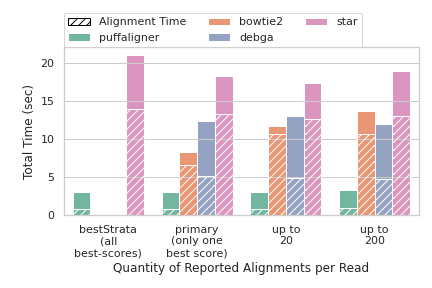
\includegraphics[width=0.8\columnwidth, type=png,ext=.png,read=.png]
    {Figures/puff/microbiome_single_time}{}}
    %{aligning a single strain sample averaged over all three samples.}}
    %\label{sfig:single_align}
    \hfill
    \subfloat[] %\centering
    {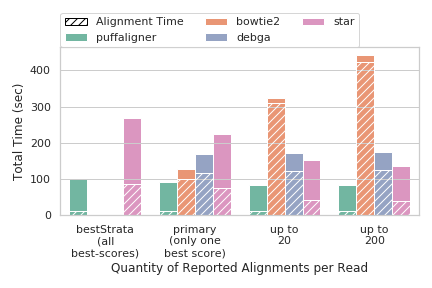
\includegraphics[width=0.8\columnwidth, type=png,ext=.png,read=.png]
    {Figures/puff/microbiome_bulk_time}{}}
    %{aligning a mock experiment simulated from bulk read sample SRR10948222.}}
    %\label{sfig:bulk_align}
    \caption[Time performance of different aligners on the microbiome
    experiments]{Time performance of different aligners on the two microbiome
    experiments. In (a), the results are averaged
    over the three alignment processes for the samples covid19, sars, and
    bat200, each having $\sim1M$ paired-end reads.
    The performance shown in (b) is for aligning reads
    in the mock sample simulated from SRR10948222 with $5M$ paired-end reads.
    As shown in the bulk experiment, the alignment for \bt
    increases when asking for more alignments per read while the other tools show a
    constant alignment time scaling over number of reads. The dashed area
    shows fraction of the time spent purely on aligning reads where the
    remaining portion is the time required for index loading. \puffaligner is 
    the fastest tool in this experiment, yet most of its time is still dedicated
    to loading the index.}
    \label{fig:alignment_performance}
    \vspace{-0.2in}
\end{figure}



\subsection{Scalability}
\begin{figure}%[h!]
    \centering
    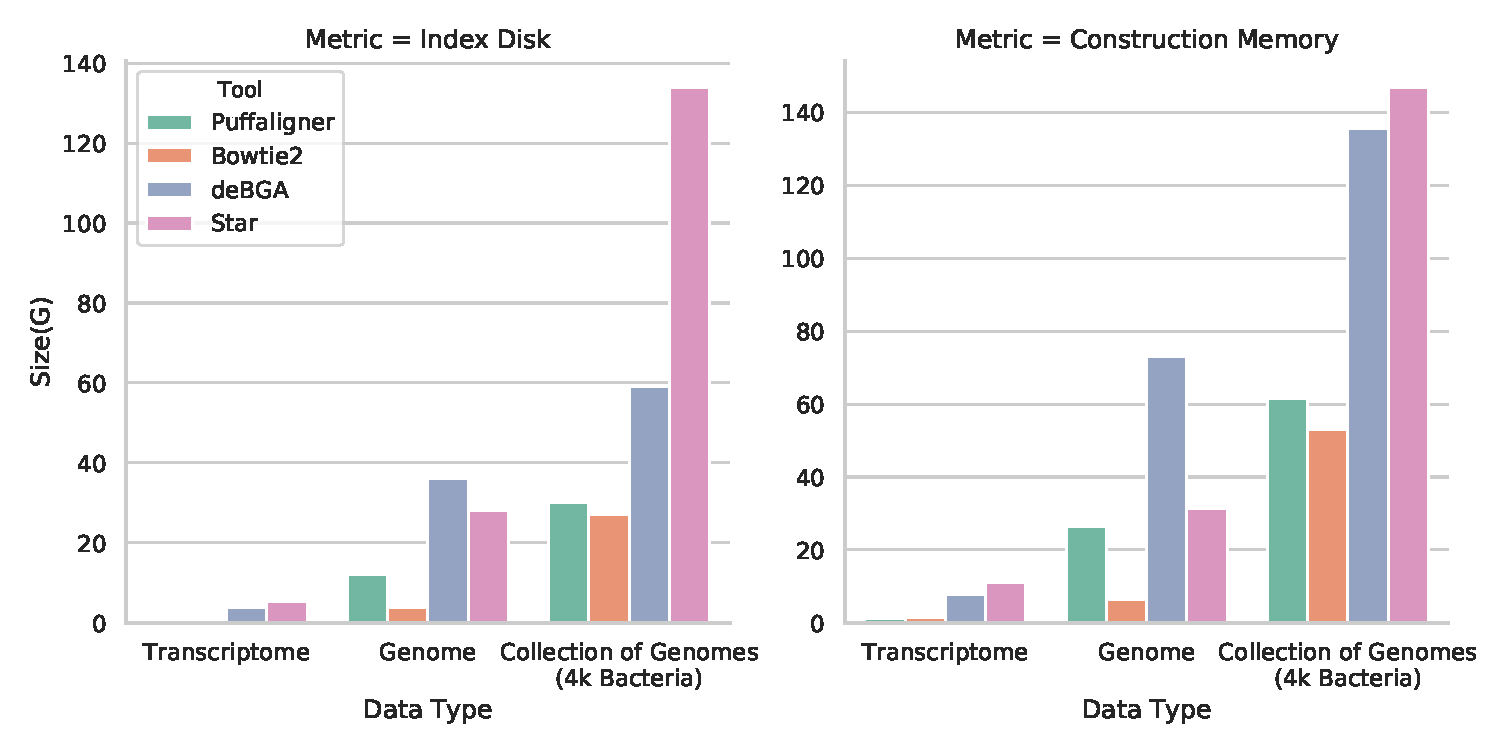
\includegraphics[width=0.8\columnwidth,type=pdf,ext=.pdf,read=.pdf]
    {Figures/puff/indexSizeScale}
    \caption[scalability of different aligners - memory]
    {Scalability of different tools over the final index disk space, construction 
    memory, for three different datasets, human transcriptome (gencode version 33), 
    human genome (GRCh38 primary assembly), and collection of genomes (4000
    random bacterial complete genomes). All tools are run with 16 threads.}
    \label{sfig:size}
\end{figure}
\begin{figure}%[h!]
    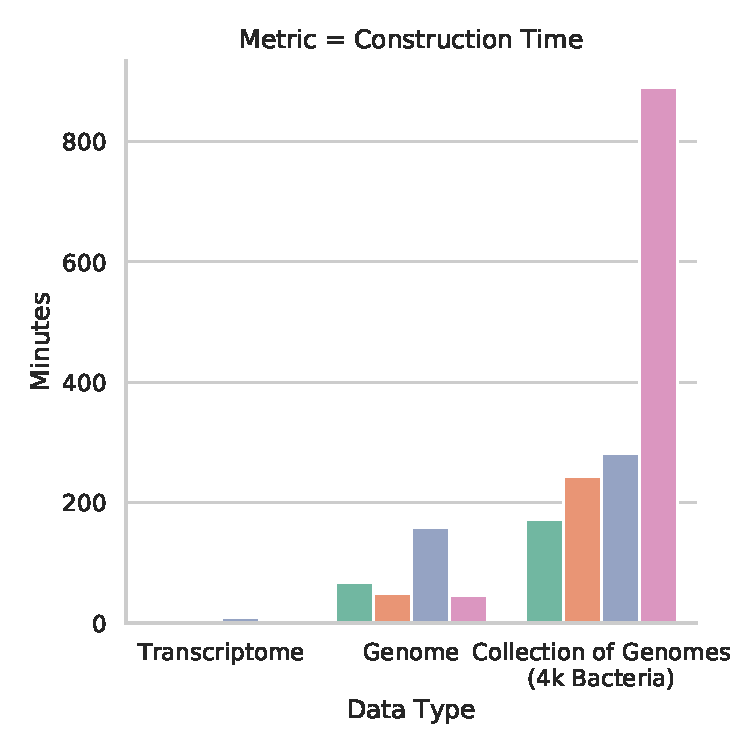
\includegraphics[width=0.8\columnwidth,type=pdf,ext=.pdf,read=.pdf]
    {Figures/puff/indexTimeScale}
    \caption[scalability of different aligners - time]
    {Scalability of different tools over the construction running time for three
    different datasets, human transcriptome (gencode version 33), human
    genome (GRCh38 primary assembly), and collection of genomes (4000
    random bacterial complete genomes). All tools are run with 16 threads.}
    \label{sfig:construction}
    \vspace{-0.2in}
\end{figure}

~\Cref{sfig:construction} and~\cref{sfig:size} represents how the construction time and
index size of each tool scales over different types of sequences. 
The trend shows the effect of database size as well as redundancy and sequence similarity on
the scalability of each of the tools. Tools such as \puffaligner and
\debga, which build a \dbg based index on the input sequence,
specifically compress similar sequences into unitigs and therefore
scale well for databases with high redundancy such as microbiomes. It is 
worth mentioning that \bt requires a switch from a $32$-bit
index to a $64$-index as the total count of the input bases
increases, which is another reason why the size is growing super-linearly.

\subsection{Discussion \& Conclusion}
\label{sec:conclusion}

In this section we introduced \puffaligner, an aligner suitable for the
contiguous alignment of short-read sequencing data. We demonstrate its
use in aligning DNA-seq reads to the genome of a single species, aligning RNA-seq reads
to the transcriptome, and aligning DNA-seq reads from metagenomic samples to a 
large collection of references. It is built on top of the \pufferfish index, which constructs
a \ccdbg using the input reference sequences. \puffaligner begins read
alignment by collecting unique maximal exact matches, querying \kmers from the
read in the \pufferfish index. The aligner then chains together the collected
uni-\mems using a dynamic programming approach, choosing the chains with the
highest coverage as potential alignment positions for the reads. Finally,
\puffaligner is able to efficiently compute alignment,
exploiting information from long matches in the chains and making use of an 
alignment cache to avoid redundant work.

We compared the accuracy and efficiency of \puffaligner against two
widely-used alignment tools, \bt and \st, that perform unspliced and
(optionally) spliced alignments of reads, respectively. We also compare
the results against \debga, an aligner that also utilizes an index built
over the compacted \dbg.

We analyze the performance of these tools on both simulated and
experimental DNA and RNA sequencing datasets. The accuracy of
\puffaligner is comparable to \bt, which exhibits very high  
alignment. \puffaligner generally performs better than \st and \debga
(though, unlike \st, none of these other tools currently support spliced read
alignment). In terms of speed and memory, \puffaligner reaches a tradeoff
between the relatively high memory usage of \st and \debga and the slower
speed of \bt. Hence, while the memory requirement of \puffaligner is more
than that of \bt, the speed gain is significant.  In the tests performed 
in this manuscript, \puffaligner is almost always the fastest tool (
with the exception being that \st is faster when aligning unspliced 
DNA-seq reads to a single human genome).

An additional advantage of the \pufferfish index utilized in \puffaligner
is that it can be built on a mixed collection of genomes, transcriptomes,
or both. This feature is already utilized in a specific pipeline for
RNA-seq quantification that makes use of a joint index over the genome 
and transcriptome~\citep{srivastava2019alignment}. The analysis shows 
that specificity of alignments in such a case can be improved by filtering 
from quantification reads that are better aligned to some genomic locus 
that is not present in the transcriptome.

Furthermore, the nature of the \pufferfish index, that explicitly
factorizes out highly-repetive sequence, coupled with the fast (and
repetition-aware) alignment procedure of \puffaligner makes it a
particularly useful for indexing and aligning to a highly similar
collection of sequences. This potentially makes it a good match 
for metagenomic analyses.

We have provided a proof of concept for such a \puffaligner-based
metagenomic analysis pipeline, and plan to build a more sophisticated 
and fully-featured metagenomic analysis framework around \puffaligner 
in the future. 